\documentclass[11pt,a4paper]{report}
\input{preamble}
\input{macros}
\usepackage{bht-cover-page}
\usepackage{layout}
\selectlanguage{ngerman} % or english 

\begin{document}

% Cover

\submissionDate{\today}
\coverPageLanguage{de}  % or {en}
\thesisTitle{Konzeption, Umsetzung und Evaluation einer mobilen Anwendung für Tierarztpraxen}
\thesisSubtitle{Vorlage für eine Bachelorarbeit bei Siamak Haschemi an der BHT}
\authorName{Aziz Erol}
\studentId{102607}
\department{VI - Informatik und Medien}
\degreeType{Bachelor of Science (B. Sc.)}
\degreeProgram{Medieninformatik}
\supervisorField{
  \begin{tabular}{lr}
    \multicolumn{2}{l}{\textbf{Reviewer}}\\
    Prof.~Dr.~Siamak Haschemi\\
    Prof.~Dr.~Dragan Macos
  \end{tabular}
}

\maketitle

% Abstract

\pagenumbering{roman}
\begin{abstract}

Die Digitalisierung der Terminverwaltung im veterinärmedizinischen Bereich weist im
Vergleich zur Humanmedizin noch erhebliche Lücken auf. Bestehende Softwarelösungen
decken entweder ausschließlich interne Praxisverwaltungsfunktionen ab oder bieten
einen zu breiten Funktionsumfang, der über die reine Terminverwaltung hinausgeht.
Im Rahmen dieser Arbeit wird daher untersucht, wie sich eine plattformübergreifende
Terminverwaltungsanwendung für Tierhalter im Kontext von Veterinärmedizinpraxen
konzipieren, umsetzen und hinsichtlich ihrer Funktionalität und Usability evaluieren
lässt.

Methodisch folgt die Arbeit dem Ansatz des Design Science Research nach Hevner et al.,
da im Mittelpunkt die Konstruktion eines Artefakts steht, das ein praxisrelevantes
Problem löst. Als Ergebnis wurde die mobile Anwendung \textit{petappoint} entwickelt.
Die Anwendung wurde mit React Native und Expo umgesetzt und ermöglicht Tierhaltern
die Registrierung, die Verwaltung von Haustierprofilen, die Suche nach
Tierarztpraxen sowie die Buchung und Stornierung von Terminen.

Zur Evaluation wurde eine aufgabenbasierte Nutzerstudie mit 20 Teilnehmenden
durchgeführt, die gleichmäßig auf iOS und Android aufgeteilt wurden. Alle
Teilnehmenden schlossen sämtliche Aufgaben erfolgreich ab, was einer Erfolgsrate
von 100\,\% entspricht. Der durchschnittliche System Usability Scale\,(SUS)-Score
von 94,34 entspricht der Note~A und belegt eine hohe wahrgenommene
Gebrauchstauglichkeit auf beiden Plattformen. Die Ergebnisse zeigen, dass eine
fokussierte, plattformübergreifende Terminverwaltungslösung im veterinärmedizinischen
Bereich sowohl technisch umsetzbar als auch von der Zielgruppe als intuitiv nutzbar
bewertet wird.

\end{abstract}

\cleardoublepage
\thispagestyle{empty}

\section*{Eigenständigkeitserklärung}

Ich, Aziz Erol, versichere hiermit, dass ich die vorliegende Arbeit selbstständig verfasst und keine anderen als die angegebenen Quellen und Hilfsmittel
benutzt habe, wobei ich alle wörtlichen und sinngemäßen Zitate als solche gekennzeichnet habe.

Es wurden folgende KI-Tools verwendet: Claude Sonnet 4.6 (Anthropic), Perplexity Sonar 2 (Perplexity AI) sowie DeepL (DeepL SE). Etwaige durch die KI vorgenommenen Änderungen
und Empfehlungen wurden von mir kritisch geprüft und gegebenenfalls angepasst, um die wissenschaftliche Integrität und die Originalität der Arbeit sicherzustellen.

Diese Arbeit wurde bisher in gleicher oder ähnlicher Form keiner anderen  Prüfungsbehörde vorgelegt und auch nicht veröffentlicht.

\bigskip
Berlin, den \today

\bigskip
\bigskip
\noindent\rule{6cm}{0.4pt}

\addtocounter{page}{-1}
\cleardoublepage













% Table of Contents

\hypertarget{toc}{}     % for "table of content squares"
\tableofcontents

% Indexes

\EnableTocSquares
\listoffigures
\cleardoublepage
\listoftables
\cleardoublepage

% List of Abbreviations / Abkürzungsverzeichnis
\printglossaries
\cleardoublepage

% Main Content

\pagenumbering{arabic}
\chapter{Einleitung}

\section{Hintergrund und Motivation}

Die Digitalisierung ist heute allgegenwärtig und stellt einen unverzichtbaren Bestandteil 
der Kommunikation zwischen Unternehmen und Kunden dar. Insbesondere im Bereich der 
Humanmedizin wird deutlich, wie digitale Technologien im Kontext der Kommunikation einen 
Vorteil bieten. Unternehmen wie Doctolib haben bereits früh das Ziel gesetzt, die 
Terminverwaltung zwischen Arztpraxen und Patienten durch den Einsatz digitaler 
Terminverwaltungssysteme effizienter und nutzerfreundlicher zu gestalten. Dieses Ziel haben 
sie weitgehend erreicht: Die digitale Terminbuchung ist heute nicht mehr wegzudenken und 
wird von vielen Patienten als entscheidender Faktor für die Inanspruchnahme von ärztlichen 
Leistungen wahrgenommen.

Vor diesem Hintergrund drängt sich die Frage auf, wie die Situation im 
veterinärmedizinischen Bereich aussieht. In Deutschland gibt es rund 10.500 
Tierarztpraxen, von denen über die Hälfte Kleintierpraxen sind, die sich auf Haustiere 
spezialisiert haben (Bundestierärztekammer, 2024). Viele Tierarztpraxen nutzen bereits 
Praxisverwaltungssoftware, um interne Aufgaben wie Terminplanung, Abrechnung und 
Dokumentation zu organisieren. Allerdings existiert bisher kein etabliertes Unternehmen, 
das den Markt für die Terminverwaltung zwischen Tierbesitzern und Tierarztpraxen ähnlich 
beherrscht wie etwa Doctolib in der Humanmedizin.

Zudem gibt es bisher keine repräsentativen Studien, die ermitteln, wie viele 
Tierarztpraxen bereits eine Terminverwaltungssoftware mit Online-Terminbuchung für 
Tierbesitzer in ihren Alltag integriert haben. Dennoch lassen Marktberichte darauf 
schließen, dass sich die Digitalisierung der Veterinärmedizin der der Humanmedizin 
zunehmend annähert: Der globale Markt für Veterinärpraxis-Managementsoftware wird für 
2023/24 auf etwa 1,8 bis 2,0~Milliarden US-Dollar geschätzt und soll bis etwa 2032 auf 
rund 3,2~Milliarden US-Dollar wachsen, mit einer jährlichen Wachstumsrate von etwa 6--7~\%. 
Auf dieser Grundlage lässt sich plausibel argumentieren, dass die Digitalisierung der 
Veterinärbranche sich in jeglichen digitalen Bereichen weiterentwickeln wird -- damit ist 
auch die Terminverwaltung zwischen Tierarztpraxen und Tierbesitzern gemeint.

\section{Zielsetzung}

Vor diesem Hintergrund zielt die vorliegende Bachelorarbeit darauf ab, eine 
Terminverwaltungssoftware zu konzipieren, umzusetzen und zu evaluieren, um 
Tierbesitzerinnen die Terminbuchung zu erleichtern. Die Software soll ermöglichen, 
Haustiere anzulegen, Tierpraxen in der Nähe zu suchen und Termine jederzeit online zu 
buchen. Der zentrale Mehrwert liegt in der flexiblen, ortsunabhängigen Online-Terminvergabe, 
die die Telefonlast reduziert und eine einfache Verwaltung für Nutzende bietet. Im 
Vergleich zu bestehenden Lösungen hebt sich \textit{Petappoint} durch seinen Fokus auf 
die Terminverwaltung ab. Onlineberatungsgespräche oder das Tracken der Tiergesundheit 
sind nicht Teil der Software.

Die Arbeit grenzt sich bewusst ab: Eine Tierpraxenansicht mit Funktionen für das Personal 
wird nicht umgesetzt. Der Schwerpunkt liegt ausschließlich auf der Konzeption, Umsetzung und 
Evaluation der Software aus Sicht der Tierbesitzer.

\chapter{Anforderungsermittlung}

In der Einleitung wurde deutlich, dass \textit{petappoint} eine fokussierte Lösung für die Terminverwaltung zwischen Tierhaltern und Tierarztpraxen darstellt. Um diese Lösung zielgerichtet umzusetzen, folgt die Anforderungsermittlung dieser Arbeit den Prinzipien des Requirements Engineering. Das ist eine Disziplin, deren Ziel es ist, die Wünsche und Bedürfnisse aller Stakeholder zu verstehen und zu dokumentieren \cite[S.~3]{pohl2021}. Stakeholder sind wiederum Personen oder Organisationen, die Einfluss auf die Anforderungen des Systems haben \cite[S.~2]{pohl2021}. Dazu zählen auch die Nutzenden von petappoint. Eine Anforderung wird dabei als ein notwendiges Bedürfnis eines Stakeholders angesehen, die die Anwendung erfüllen muss \cite[S.~1]{pohl2021}.

Die Analyse der Anforderungen bildet die Grundlage für Konzeption und Entwicklung der vorliegenden Anwendung und Arbeit. Ziel dieses Kapitels ist es, ein vollständiges Bild der Anforderungen zu erarbeiten und diese strukturiert zu dokumentieren.

Zu Beginn wird die Zielgruppe der Anwendung identifiziert und charakterisiert. Darauf aufbauend werden die relevanten funktionalen sowie nicht funktionalen Anforderungen hergeleitet und gegliedert dargestellt. Abschließend werden ausgewählte Anforderungen durch Use Cases konkretisiert und in ihrem praktischen Kontext veranschaulicht.

\section{Zielgruppe}
Die Anwendung richtet sich an zwei primäre Zielgruppen: Tierhalter sowie Tierarztpraxen. Im Rahmen der Analyse bestehender Softwarelösungen in Kapitel 2 wurde deutlich, dass in diesem Bereich keine spezialisierte Terminverwaltungslösung existiert, die beide gleichermaßen adressiert.

Die Anforderungen beider Zielgruppen lassen sich durch folgende Aspekte charakterisieren:

\textbf{Tierhalter}

\begin{itemize}
    \item \textbf{Einfache Bedienbarkeit:} Da die Nutzende in der Regel über keine spezifischen technischen Vorkenntnisse verfügen, muss die Anwendung intuitiv bedienbar sein und ohne umfangreiche Einarbeitung genutzt werden können.
    \item \textbf{Verfügbarkeit rund um die Uhr:} Da berufstätige Tierhalter häufig tagsüber keine Möglichkeit haben, telefonisch einen Termin zu vereinbaren, muss die Buchung zu jeder Tages- und Nachtzeit möglich sein.
    \item \textbf{Haustierzentrierte Verwaltung:} Die Anwendung muss die Anlage mehrerer Haustierprofile mit relevanten Informationen wie Tierart, Rasse und Geburtsdatum unterstützen.
    \item \textbf{Benachrichtigungen:} Automatische Erinnerungen vor bevorstehenden Terminen per E-Mail oder Push-Benachrichtigung sollen vergessene Arztbesuche reduzieren.
    \item \textbf{Datensicherheit:} Da personenbezogene Daten sowie Gesundheitsdaten der Tiere verarbeitet werden, dürfen diese ausschließlich für die jeweiligen Nutzenden zugänglich sein.
\end{itemize}

\textbf{Tierarztpraxen}

\begin{itemize}
    \item \textbf{Digitale Kalender- und Terminverwaltung:} Praxen benötigen ein flexibles System zur Definition von Öffnungszeiten, Terminarten und Kapazitäten, das eine manuelle Terminvergabe per Telefon überflüssig macht.
    \item \textbf{Übersichtliche Tagesplanung:} Ein Dashboard mit Tages- und Wochenansicht aller gebuchten Termine inklusive relevanter Patientendaten ist für einen reibungslosen Praxisablauf erforderlich.
    \item \textbf{Praxisprofil und Auffindbarkeit:} Praxen müssen ihre Leistungen, behandelten Tierarten und Spezialisierungen pflegen können, um von Tierhaltern gezielt gefunden zu werden.
    \item \textbf{Plattformunabhängigkeit:} Die Anwendung soll über gängige Webbrowser nutzbar sein, ohne dass eine lokale Installation erforderlich ist.
\end{itemize}

Zusammenfassend zeigt die Zielgruppenanalyse, dass die Anwendung sowohl für nicht technische Nutzende auf der Seite der Tierhalter als auch für den professionellen Einsatz in tierärztlichen Praxen konzipiert werden muss. Die Berücksichtigung beider Perspektiven ist entscheidend für die Akzeptanz und den nachhaltigen Erfolg des Systems.

\section{Funktionale Anforderungen}

Grundlegend wird zwischen zwei Arten von Anforderungen unterschieden auf die man Einfluss hat: Funktionale Anforderungen und Nicht Funktionale Anforderungen. Funktionale Anforderungen (FA) beschreiben, welche Funktionen und Fähigkeiten das System den Nutzenden zur Verfügung stellen soll \cite[S.~3]{pohl2021}. Zur eindeutigen Formulierung der funktionalen Anforderungen werden 
Satzschablonen eingesetzt. Eine Satzschablone ist ein Bauplan für die 
syntaktische Struktur einer einzelnen Anforderung in natürlicher Sprache 
\cite[S.~71]{pohl2021}. Die funktionalen Anforderungen wurden aus der 
Perspektive beider Zielgruppen abgeleitet:

\textbf{Tierhalter}

\begin{itemize}
    \item \textbf{FA\#01} Die mobile Anwendung \textbf{muss} Nutzenden 
    ermöglichen, sich zu registrieren und anzumelden.

    \item \textbf{FA\#02} Die mobile Anwendung \textbf{muss} Nutzenden 
    ermöglichen, Haustierprofile zu erstellen und zu verwalten.

    \item \textbf{FA\#03} Die mobile Anwendung \textbf{muss} Nutzenden 
    ermöglichen, Tierarztpraxen zu suchen und zu filtern.

    \item \textbf{FA\#04} Die mobile Anwendung \textbf{muss} Nutzenden 
    ermöglichen, verfügbare Termine einzusehen und zu buchen.

    \item \textbf{FA\#05} Die mobile Anwendung \textbf{muss} Nutzenden 
    ermöglichen, gebuchte Termine einzusehen und zu stornieren.

    \item \textbf{FA\#06} Die mobile Anwendung \textbf{muss} Nutzende 
    über Änderungen an ihren Terminen benachrichtigen.
\end{itemize}

\textbf{Tierarztpraxen}

\begin{itemize}
    \item \textbf{FA\#07} Die mobile Anwendung \textbf{muss} 
    Tierarztpraxen ermöglichen, ihr Profil und ihre Verfügbarkeiten 
    zu verwalten.

    \item \textbf{FA\#08} Die mobile Anwendung \textbf{muss} 
    Tierarztpraxen ermöglichen, eingehende Buchungen einzusehen 
    und zu verwalten.
\end{itemize}

\section{Nicht funktionale Anforderungen}

Nicht funktionale Anforderungen sind Qualitätsanforderungen, die sich auf 
die Qualitätsmerkmale des Systems beziehen \cite[S.~4] {pohl2021}.

\begin{itemize}
    \item \textbf{NFA\#01} Die mobile Anwendung muss auf gängigen iOS- und Android-Geräten nutzbar sein.
\end{itemize}

\section{Use Cases}

Use Cases stellen das Verhalten eines Systems aus dem Blickwinkel der Nutzenden dar. Sie beschreiben, wie das System auf eine Interaktion reagiert, welche Ziele damit verfolgt werden und welche alternativen Abläufe dabei auftreten können \cite[S.~15]{cockburn2001}. Aufgrund ihrer textuellen Form eignen sie sich besonders zur klaren und verständlichen Beschreibung funktionaler Anforderungen und ermöglichen eine verständliche Kommunikation ohne besondere fachliche Vorkenntnisse \cite[S.~15]{cockburn2001}. Zur besseren Dokumentation und zur Vollständigkeit werden Sie im Folgenden durch ein Use-Case-Diagramm ergänzt \cite[S.~75]{pohl2021}.

\subsection{Use Case Diagramm}
\begin{landscape}
\begin{figure}[H]
    \centering
    \includesvg[width=0.4\linewidth]{figures/use-case-diagram.svg}
    \caption{Use-Case-Diagramm petappoint}
    \label{fig:usecase-gesamt}
\end{figure}
\end{landscape}

\subsection{Haustier anlegen}

\renewcommand{\arraystretch}{1.5}
\begin{tabular}{|p{5cm}|p{9.2cm}|}
\hline
\textbf{Name} & UC-01: Haustier anlegen \\
\hline
\textbf{Kurzbeschreibung} & Der Tierhalter legt ein neues Haustierprofil 
in der Anwendung an. \\
\hline
\textbf{Akteure} & Tierhalter \\
\hline
\textbf{Vorbedingungen} & 
Der Tierhalter ist eingeloggt. \\
\hline
\textbf{Auslösendes Ereignis} & Der Tierhalter möchte ein neues Haustier 
in der Anwendung erfassen. \\
\hline
\textbf{Hauptszenario} &
1. Der Tierhalter öffnet den Tab „Meine Haustiere". \newline
2. Der Tierhalter tippt auf „Haustier hinzufügen". \newline
3. Die Anwendung öffnet einen neuen Screen mit Eingabefeldern. \newline
4. Der Tierhalter gibt die Daten des Haustieres ein. \newline
5. Der Tierhalter tippt optional auf „Profilbild hinzufügen" und 
wählt ein Bild über die Gerätekamera oder Galerie aus. \newline
6. Der Tierhalter tippt auf „Haustier anlegen". \newline
7. Die Anwendung validiert die Daten. \newline
8. Die Anwendung speichert das Haustier. \newline
9. Der Tierhalter wird zum Tab 'Meine Haustiere' weitergeleitet. \\
\hline
\textbf{Alternativszenario} &
1. Pflichtfelder sind leer $\rightarrow$ Der Button bleibt deaktiviert. \newline
2. Der Tierhalter verweigert den Kamerazugriff $\rightarrow$ Die Anwendung 
zeigt einen Hinweis und erlaubt die Auswahl aus der Galerie. \newline
3. Der Tierhalter verweigert auch den Galerie-Zugriff $\rightarrow$ Das Haustier kann auch ohne Profilbild angelegt werden. \\
\hline
\textbf{Nachbedingungen} &
Das neue Haustier ist unter „Meine Haustiere" sichtbar. \\
\hline
\end{tabular}

\subsection{Haustier bearbeiten}
\renewcommand{\arraystretch}{1.5}
\begin{tabular}{|p{5cm}|p{9.2cm}|}
\hline
\textbf{Name} & UC-02: Haustier bearbeiten \\
\hline
\textbf{Kurzbeschreibung} & Der Tierhalter bearbeitet die Daten eines 
bestehenden Haustierprofils. \\
\hline
\textbf{Akteure} & Tierhalter \\
\hline
\textbf{Vorbedingungen} & 
Der Tierhalter ist eingeloggt. \newline
Der Tierhalter hat mindestens ein Haustier angelegt. \\
\hline
\textbf{Auslösendes Ereignis} & Der Tierhalter möchte die Daten eines 
Haustieres aktualisieren. \\
\hline
\textbf{Hauptszenario} &
1. Der Tierhalter öffnet den Tab „Meine Haustiere". \newline
2. Der Tierhalter tippt auf „Bearbeiten" in der Karte des gewünschten 
Haustieres. \newline
3. Die Anwendung öffnet einen neuen Screen mit den aktuellen Daten 
des Haustieres. \newline
4. Der Tierhalter ändert die gewünschten Daten. \newline
5. Der Tierhalter tippt optional auf „Profilbild ändern" und wählt 
ein neues Bild über die Gerätekamera oder Galerie aus. \newline
6. Der Tierhalter tippt auf „Speichern". \newline
7. Die Anwendung validiert die Daten. \newline
8. Die Anwendung speichert die Änderungen und leitet zurück zu 
„Meine Haustiere". \\
\hline
\textbf{Alternativszenario} &
1. Pflichtfelder sind leer $\rightarrow$ Der Button bleibt deaktiviert. \newline
2. Der Tierhalter verweigert den Kamerazugriff $\rightarrow$ Die Anwendung 
zeigt einen Hinweis und erlaubt die Auswahl aus der Galerie. \newline
3. Der Tierhalter verweigert auch den Galerie-Zugriff $\rightarrow$ Die 
Anwendung zeigt einen Hinweis und das Profilbild bleibt unverändert. \\
\hline
\textbf{Nachbedingungen} &
Das Haustier wird unter „Meine Haustiere" mit den aktualisierten 
Daten angezeigt. \\
\hline
\end{tabular}

\subsection{Haustier löschen}
\renewcommand{\arraystretch}{1.5}
\begin{tabular}{|p{5cm}|p{9.2cm}|}
\hline
\textbf{Name} & UC-03: Haustier löschen \\
\hline
\textbf{Kurzbeschreibung} & Der Tierhalter löscht ein bestehendes 
Haustierprofil aus der Anwendung. \\
\hline
\textbf{Akteure} & Tierhalter \\
\hline
\textbf{Vorbedingungen} & 
Der Tierhalter ist eingeloggt. \newline
Der Tierhalter hat mindestens ein Haustier angelegt. \\
\hline
\textbf{Auslösendes Ereignis} & Der Tierhalter möchte ein Haustierprofil 
dauerhaft entfernen. \\
\hline
\textbf{Hauptszenario} &
1. Der Tierhalter öffnet den Tab „Meine Haustiere". \newline
2. Der Tierhalter tippt auf Bearbeiten im Bereich des gewünschten 
Haustieres. \newline
3. Der Tierhalter tippt auf „Haustier löschen". \newline
4. Die Anwendung öffnet einen Bestätigungs-Bottom-Sheet mit einer 
Warnmeldung. \newline
5. Der Tierhalter bestätigt den Löschvorgang. \newline
6. Die Anwendung löscht das Haustierprofil. \newline
7. Der Tierhalter wird zum Tab „Meine Haustiere" weitergeleitet. \\
\hline
\textbf{Alternativszenario} &
1. Der Tierhalter bricht den Bestätigungs-Bottom-Sheet ab 
$\rightarrow$ Das Haustier bleibt erhalten. \\
\hline
\textbf{Nachbedingungen} &
Das gelöschte Haustier ist nicht mehr unter „Meine Haustiere" sichtbar. \\
\hline
\end{tabular}

\subsection{Termin buchen}
\renewcommand{\arraystretch}{1.5}
\begin{tabular}{|p{5cm}|p{9.2cm}|}
\hline
\textbf{Name} & UC-04: Termin buchen \\
\hline
\textbf{Kurzbeschreibung} & Der Tierhalter bucht einen Termin bei einer 
Tierarztpraxis für sein Haustier. \\
\hline
\textbf{Akteure} & Tierhalter \\
\hline
\textbf{Vorbedingungen} & 
Der Tierhalter ist eingeloggt. \newline
Der Tierhalter hat mindestens ein Haustier angelegt. \\
\hline
\textbf{Auslösendes Ereignis} & Der Tierhalter möchte einen Tierarzttermin 
für sein Haustier vereinbaren. \\
\hline
\textbf{Hauptszenario} &
1. Der Tierhalter tippt auf „Termin buchen". \newline
2. Der Tierhalter gibt optional einen Ort, ein Haustier und eine 
Behandlungsart an. \newline
3. Der Tierhalter tippt auf „Suchen". \newline
4. Die Anwendung zeigt passende Tierarztpraxen in der Nähe in einer 
scrollbaren Liste an. \newline
5. Der Tierhalter tippt auf eine Praxis. \newline
6. Die Anwendung zeigt die Praxisdetails sowie verfügbare Termine 
in einer scrollbaren Kalenderansicht. \newline
7. Der Tierhalter wählt ein Datum und eine Uhrzeit aus. \newline
8. Der Tierhalter tippt auf „Bestätigen". \newline
9. Die Anwendung zeigt eine Buchungsübersicht. \newline
10. Der Tierhalter tippt auf „Termin buchen". \newline
11. Die Anwendung speichert den Termin. \newline
12. Der Tierhalter erhält eine Push-Benachrichtigung als 
Buchungsbestätigung. \newline
13. Der Tierhalter wird zum Tab „Meine Termine" weitergeleitet. \\
\hline
\textbf{Alternativszenario} &
1. Kein Ort angegeben $\rightarrow$ Die Anwendung ermittelt den 
Standort automatisch per GPS und zeigt nahegelegene Praxen. \newline
2. Der Tierhalter verweigert den GPS-Zugriff $\rightarrow$ Die Anwendung 
fordert den Tierhalter zur manuellen Ortseingabe auf. \newline
3. Keine freien Termine verfügbar $\rightarrow$ Die Anwendung zeigt 
einen entsprechenden Hinweis. \\
\hline
\textbf{Nachbedingungen} &
Der gebuchte Termin ist unter „Meine Termine" sichtbar. \\
\hline
\end{tabular}

\subsection{Termin bearbeiten}
\renewcommand{\arraystretch}{1.5}
\begin{tabular}{|p{5cm}|p{9.2cm}|}
\hline
\textbf{Name} & UC-05: Termin bearbeiten \\
\hline
\textbf{Kurzbeschreibung} & Der Tierhalter ändert einen bestehenden 
gebuchten Termin. \\
\hline
\textbf{Akteure} & Tierhalter \\
\hline
\textbf{Vorbedingungen} & 
Der Tierhalter ist eingeloggt. \newline
Der Tierhalter hat mindestens einen gebuchten Termin. \\
\hline
\textbf{Auslösendes Ereignis} & Der Tierhalter möchte Datum, Uhrzeit 
oder Haustier eines Termins ändern. \\
\hline
\textbf{Hauptszenario} &
1. Der Tierhalter öffnet den Tab „Meine Termine". \newline
2. Der Tierhalter tippt auf den gewünschten Termin. \newline
3. Der Tierhalter tippt auf „Termin bearbeiten". \newline
4. Die Anwendung öffnet einen neuen Screen mit den aktuellen 
Termindaten. \newline
5. Der Tierhalter ändert die gewünschten Daten in einer 
scrollbaren Kalenderansicht. \newline
6. Der Tierhalter tippt auf „Speichern". \newline
7. Die Anwendung validiert die Daten. \newline
8. Die Anwendung speichert die Änderungen und leitet zurück 
zu „Meine Termine". \newline
9. Der Tierhalter erhält eine Push-Benachrichtigung als 
Bestätigung der Änderung. \\
\hline
\textbf{Alternativszenario} &
1. Der gewünschte Termin ist nicht mehr verfügbar $\rightarrow$ 
Die Anwendung zeigt eine Fehlermeldung und schlägt alternative 
freie Termine vor. \\
\hline
\textbf{Nachbedingungen} &
Der Termin wird unter „Meine Termine" mit den aktualisierten 
Daten angezeigt. \\
\hline
\end{tabular}

\subsection{Termin stornieren}
\renewcommand{\arraystretch}{1.5}
\begin{tabular}{|p{5cm}|p{9.2cm}|}
\hline
\textbf{Name} & UC-06: Termin stornieren \\
\hline
\textbf{Kurzbeschreibung} & Der Tierhalter storniert einen bestehenden 
gebuchten Termin. \\
\hline
\textbf{Akteure} & Tierhalter \\
\hline
\textbf{Vorbedingungen} & 
Der Tierhalter ist eingeloggt. \newline
Der Tierhalter hat mindestens einen gebuchten Termin. \\
\hline
\textbf{Auslösendes Ereignis} & Der Tierhalter möchte einen gebuchten 
Termin absagen. \\
\hline
\textbf{Hauptszenario} &
1. Der Tierhalter öffnet den Tab „Meine Termine". \newline
2. Der Tierhalter tippt auf den gewünschten Termin. \newline
3. Der Tierhalter tippt auf „Termin stornieren". \newline
4. Die Anwendung öffnet einen Bestätigungs-Bottom-Sheet mit 
einer Warnmeldung. \newline
5. Der Tierhalter bestätigt die Stornierung. \newline
6. Die Anwendung hebt die Buchungsverbindung auf und gibt 
den Termin frei. \newline
7. Der Tierhalter erhält eine Push-Benachrichtigung als 
Bestätigung der Stornierung. \newline
8. Der Tierhalter wird zum Tab „Meine Termine" weitergeleitet. \\
\hline
\textbf{Alternativszenario} &
1. Der Tierhalter bricht den Bestätigungs-Bottom-Sheet ab 
$\rightarrow$ Der Termin bleibt gebucht. \\
\hline
\textbf{Nachbedingungen} &
Der stornierte Termin ist nicht mehr unter „Meine Termine" sichtbar. \\
\hline
\end{tabular}

\subsection{Buchungen einsehen}
\renewcommand{\arraystretch}{1.5}
\begin{tabular}{|p{5cm}|p{9.2cm}|}
\hline
\textbf{Name} & UC-07: Buchungen einsehen \\
\hline
\textbf{Kurzbeschreibung} & Die Tierarztpraxis sieht alle gebuchten 
Termine in einer Tages- und Wochenansicht ein. \\
\hline
\textbf{Akteure} & Tierarztpraxis \\
\hline
\textbf{Vorbedingungen} & 
Die Tierarztpraxis ist eingeloggt. \\
\hline
\textbf{Auslösendes Ereignis} & Die Tierarztpraxis möchte einen 
Überblick über alle anstehenden Buchungen erhalten. \\
\hline
\textbf{Hauptszenario} &
1. Die Tierarztpraxis öffnet den Tab „Kalender". \newline
2. Die Anwendung zeigt eine Tagesansicht mit allen gebuchten 
Terminen des aktuellen Tages. \newline
3. Die Tierarztpraxis tippt auf „Wochenansicht" um zur 
Wochenübersicht zu wechseln. \newline
4. Die Tierarztpraxis tippt auf einen Termin. \newline
5. Die Anwendung zeigt die Detailansicht des Termins mit 
Name des Tierhalters, Tierart, Rasse und Behandlungsart. \\
\hline
\textbf{Alternativszenario} &
1. Keine Buchungen vorhanden $\rightarrow$ Die Anwendung zeigt 
einen entsprechenden Hinweis. \\
\hline
\textbf{Nachbedingungen} &
Die Tierarztpraxis hat einen vollständigen Überblick über 
alle anstehenden Termine. \\
\hline
\end{tabular}

\subsection{Terminslot anlegen}
\renewcommand{\arraystretch}{1.5}
\begin{tabular}{|p{5cm}|p{9.2cm}|}
\hline
\textbf{Name} & UC-08: Terminslot anlegen \\
\hline
\textbf{Kurzbeschreibung} & Die Tierarztpraxis legt einen neuen 
verfügbaren Terminslot in der Anwendung an. \\
\hline
\textbf{Akteure} & Tierarztpraxis \\
\hline
\textbf{Vorbedingungen} & 
Die Tierarztpraxis ist eingeloggt. \\
\hline
\textbf{Auslösendes Ereignis} & Die Tierarztpraxis möchte einen 
neuen Terminslot für Tierhalter verfügbar machen. \\
\hline
\textbf{Hauptszenario} &
1. Die Tierarztpraxis öffnet den Tab „Terminverwaltung". \newline
2. Die Anwendung zeigt eine scrollbare Kalenderansicht mit den 
aktuellen Terminslots. \newline
3. Die Tierarztpraxis tippt auf einen freien Zeitraum. \newline
4. Die Anwendung öffnet einen neuen Screen zur Konfiguration 
des Terminslots. \newline
5. Die Tierarztpraxis gibt Datum, Uhrzeit, Dauer und Behandlungsart an. \newline
6. Die Tierarztpraxis tippt auf „Slot speichern". \newline
7. Die Anwendung validiert die Eingaben. \newline
8. Die Anwendung speichert den Terminslot und aktualisiert 
die Kalenderansicht. \\
\hline
\textbf{Alternativszenario} &
1. Pflichtfelder sind leer $\rightarrow$ Der Button bleibt deaktiviert. \\
\hline
\textbf{Nachbedingungen} &
Der neue Terminslot ist in der Kalenderansicht sichtbar und 
für Tierhalter buchbar. \\
\hline
\end{tabular}

\subsection{Terminslot bearbeiten}
\renewcommand{\arraystretch}{1.5}
\begin{tabular}{|p{5cm}|p{9.2cm}|}
\hline
\textbf{Name} & UC-09: Terminslot bearbeiten \\
\hline
\textbf{Kurzbeschreibung} & Die Tierarztpraxis bearbeitet einen 
bestehenden Terminslot oder sperrt einen Zeitraum. \\
\hline
\textbf{Akteure} & Tierarztpraxis \\
\hline
\textbf{Vorbedingungen} & 
Die Tierarztpraxis ist eingeloggt. \newline
Es existiert mindestens ein Terminslot. \\
\hline
\textbf{Auslösendes Ereignis} & Die Tierarztpraxis möchte einen 
bestehenden Terminslot anpassen oder einen Zeitraum sperren. \\
\hline
\textbf{Hauptszenario} &
1. Die Tierarztpraxis öffnet den Tab „Terminverwaltung". \newline
2. Die Anwendung zeigt eine scrollbare Kalenderansicht mit den 
aktuellen Terminslots. \newline
3. Die Tierarztpraxis tippt auf den gewünschten Terminslot. \newline
4. Die Anwendung öffnet einen neuen Screen mit den aktuellen 
Daten des Terminslots. \newline
5. Die Tierarztpraxis ändert die gewünschten Daten. \newline
6. Die Tierarztpraxis tippt auf „Speichern". \newline
7. Die Anwendung validiert die Eingaben. \newline
8. Die Anwendung speichert die Änderungen und aktualisiert 
die Kalenderansicht. \\
\hline
\textbf{Alternativszenario} &
1. Pflichtfelder sind leer $\rightarrow$ Der Button bleibt deaktiviert. \newline
2. Die Tierarztpraxis möchte einen Zeitraum sperren $\rightarrow$ 
Die Tierarztpraxis tippt auf „Zeitraum sperren", wählt Start und 
Ende aus und bestätigt. Die Anwendung markiert den Zeitraum 
als nicht verfügbar. \\
\hline
\textbf{Nachbedingungen} &
Der Terminslot wird in der Kalenderansicht mit den aktualisierten 
Daten angezeigt. \\
\hline
\end{tabular}

\subsection{gebuchten Termin absagen}
\renewcommand{\arraystretch}{1.5}
\begin{tabular}{|p{5cm}|p{9.2cm}|}
\hline
\textbf{Name} & UC-10: Termin absagen \\
\hline
\textbf{Kurzbeschreibung} & Die Tierarztpraxis sagt einen gebuchten 
Termin ab und der betroffene Tierhalter wird automatisch benachrichtigt. \\
\hline
\textbf{Akteure} & Tierarztpraxis \\
\hline
\textbf{Vorbedingungen} & 
Die Tierarztpraxis ist eingeloggt. \newline
Es existiert mindestens ein gebuchter Termin. \\
\hline
\textbf{Auslösendes Ereignis} & Die Tierarztpraxis möchte einen 
gebuchten Termin absagen. \\
\hline
\textbf{Hauptszenario} &
1. Die Tierarztpraxis öffnet den Tab „Kalender". \newline
2. Die Tierarztpraxis tippt auf den gewünschten Termin. \newline
3. Die Tierarztpraxis tippt auf „Termin absagen". \newline
4. Die Anwendung öffnet einen Bestätigungs-Bottom-Sheet mit 
einer Warnmeldung. \newline
5. Die Tierarztpraxis bestätigt die Absage. \newline
6. Die Anwendung gibt den Terminslot frei. \newline
7. Die Anwendung benachrichtigt den betroffenen Tierhalter 
automatisch per Push-Benachrichtigung und E-Mail. \\
\hline
\textbf{Alternativszenario} &
1. Die Tierarztpraxis bricht den Bestätigungs-Bottom-Sheet ab 
$\rightarrow$ Der Termin bleibt gebucht. \\
\hline
\textbf{Nachbedingungen} &
Der abgesagte Termin ist nicht mehr in der Kalenderansicht sichtbar. \newline
Der betroffene Tierhalter wurde über die Absage informiert. \\
\hline
\end{tabular}
\chapter{Konzeption}
Die in Kapitel~2 erarbeiteten funktionalen und nicht funktionalen Anforderungen sowie die definierten Use Cases bilden die Grundlage für die Konzeption der mobilen Anwendung. In diesem Kapitel wird 
zunächst die Softwarearchitektur sowie die bestehende 
Backend-Infrastruktur als Ausgangspunkt beschrieben. Darauf aufbauend werden das Komponentendiagramm, das Navigationskonzept, die Mockups der Benutzeroberfläche sowie abschließend ein Aktivitätsdiagramm zum Terminbuchungsprozess vorgestellt.

\section{Softwarearchitektur}

Selbst innerhalb der Informatik existiert keine einheitlich
anerkannte Definition des Begriffs Softwarearchitektur~\cite[S.~1]{richards2021softwarearchitektur}. Dennoch lässt sich der Begriff inhaltlich eingrenzen. Softwarearchitektur umfasst die zentralen Grundsätze und Vorgaben, nach denen ein System gegliedert und in Komponenten sowie Schnittstellen aufgeteilt wird. Sie beschreibt zudem, wie diese Elemente untereinander und mit ihrer Umgebung
interagieren. Auf dieser Basis werden verbindliche Leitlinien für alle Phasen des Systemlebens definiert, von der Anforderungsanalyse über den Entwurf und die Implementierung bis hin zum Betrieb und zur Pflege des Systems, ebenso wie für die zugehörigen Entwicklungs- und Betriebsstrukturen~\cite[S.~21]{gharbi2020basiswissen}. Der Schwerpunkt dieses Kapitels liegt auf dem Entwurf der Software.

\subsection{Architekturübersicht}
\label{sec:architektur}

Die Architektur von \textit{petappoint} basiert auf einer Schichtenarchitektur. Bei einer Schichtenarchitektur werden
Komponenten in hierarchischen Ebenen angeordnet, wobei eine Komponente einer höheren Schicht Anfragen an eine Komponente einer niedrigeren Schicht stellen und auf deren Antwort warten kann~\cite[S.~57]{tanenbaum2007distributed}. Innerhalb dieser Struktur herrscht das Client-Server Prinzip. Der Server, der bestimmte Dienste bereitstellt, und der Client bzw. mehrere Clients, die diese Dienste durch das Senden von Anfragen in Anspruch nehmen und anschließend auf die Antwort des Servers warten~\cite[S.~79]{tanenbaum2007distributed}. Die Kommunikation zwischen Client und Server erfolgt über eine 
REST-API (Representational State Transfer). RESTful-Architekturen 
zeichnen sich dadurch aus, dass Ressourcen über ein einheitliches 
Benennungsschema identifiziert werden, alle Dienste dieselbe 
Schnittstelle mit den vier Operationen PUT, POST, GET und DELETE anbieten, Nachrichten vollständig selbstbeschreibend sind und  Dienste nach der Ausführung einer Operation keinerlei Informationen 
über den Aufrufer speichern~\cite[S.~66]{tanenbaum2007distributed}.

Die Schichtenarchitektur gliedert sich in drei Schichten: 
\begin{itemize}
    \item \textbf{Präsentationsschicht (Frontend):} Zuständig für die Darstellung 
    der Benutzeroberfläche und repräsentiert den Client des Systems.
    \item \textbf{Anwendungsschicht (Backend):} Verarbeitet eingehende 
    HTTP-Anfragen, validiert Eingabedaten und steuert den Datenbankzugriff. 
    Diese Schicht übernimmt die Rolle des Servers.
    \item \textbf{Datenschicht (Datenbank):} Verantwortlich für die Speicherung 
    und Verwaltung aller persistenten Daten der Anwendung.
\end{itemize}

Die mobile Anwendung wird in der Präsentationsschicht ergänzt und ist somit ausschließlich für die Darstellung und Nutzerinteraktion zuständig. Da das 
Backend von \textit{petappoint} im Rahmen eines vorangegangenen Projektmoduls bereits entwickelt wurde, beschränkt sich der Fokus dieser Arbeit auf die Konzeption und Umsetzung der Präsentationsschicht. Abbildung~\ref{fig:softwarearchitecture} veranschaulicht den beschriebenen Aufbau grafisch.

\begin{landscape}
\begin{figure}[H]
    \centering
    \includesvg[width=0.8\linewidth]{figures/software-architecture.svg}
    \caption{Schichtenarchitektur von petappoint}
    \label{fig:softwarearchitecture}
\end{figure}
\end{landscape}

\subsection{Bestehende Backend-Architektur als Grundlage}

Das Backend von \textit{petappoint} wurde im Rahmen eines vorangegangenen Projektmoduls entwickelt und bildet die technische Grundlage dieser Arbeit. Es stellt sämtliche Geschäftslogik und Datenhaltung bereit, auf die die mobile Anwendung über die REST-API zugreift.

Die zugrunde liegende Datenbankstruktur ist in Abbildung~\ref{fig:erdiagramm} als ER-Diagramm dargestellt. Ein Entity-Relationship-Diagramm (ER-Diagramm) ist eine grafische Methode zur Darstellung der logischen Struktur einer Datenbank. Das Modell basiert auf drei Grundkonzepten: Entitäten repräsentieren reale Objekte oder Konzepte, 
Attribute beschreiben deren Eigenschaften, und Beziehungen stellen die  Verbindungen zwischen den Entitäten dar~\cite[S.~29]{watt2014dbdesign}. Die Kardinalitäten geben dabei an, wie viele Instanzen einer Entität mit wie vielen Instanzen einer anderen Entität in Beziehung stehen können und werden in der Krähenfuß-Notation durch spezielle Symbole dargestellt, wie in Abbildung~\ref{fig:crowsfoot} gezeigt. 

Das Schema umfasst die zentralen Entitäten \textit{persons}, \textit{animals} und \textit{veterinarypractices}, die den Kern der Anwendungslogik bilden. Tierhalter werden als \textit{persons} erfasst und können keine oder mehrere Tiere (\textit{animals}) anlegen, aber ein Tier kann nicht ohne eine Person exitieren, sodass eine $1{:}n$-Beziehung zwischen \textit{persons} und \textit{animals} besteht. Jedes Tier ist dabei genau einem Tiertyp (\textit{animal\_types}) zugeordnet und ein Tiertyp kann vielen Tieren zugeordnet werden. 1 Tiertyp kann wiederum mehrere Rassen (\textit{animal\_races}) umfassen, aber mehrere 1 Rassen entstehen aus 1 Tiertyp, was einer $1{:}n$-Beziehung zwischen \textit{animal\_types} und \textit{animal\_races} entspricht.

Tierarztpraxen werden über \textit{veterinarypractices} abgebildet und stehen in einer $1{:}n$-Beziehung zu den zugehörigen Tierärzten 
(\textit{veterinarians}), da eine Praxis mehrere Tierärzte beschäftigen kann, aber eine Tierärzte genau 1 Tierarztpraxis zugeordnet werden kann. Termine werden in der Tabelle \textit{appointments} gespeichert und können optional einem Tier, einem Tierarzt sowie einer gebuchten Leistung (\textit{services}) zugeordnet werden, was einer 
$0{:}n$-Beziehung zu diesen Entitäten entspricht. Ein Termin kann allerdings nicht ohne Tierarztpraxis existieren, aber eine Praxis kann mehrere Termine besitzen, was einer $1{:}n$-Beziehung entspricht.

Darüber hinaus enthält das Schema eine Favoritenfunktion, die über die 
Relationstabelle \textit{person\_has\_favorized\_veterinarypractice} abgebildet wird. Da ein Tierhalter mehrere Praxen als Favoriten speichern kann und eine Praxis gleichzeitig von mehreren Tierhaltern favorisiert werden kann, liegt hier eine $n{:}m$-Beziehung vor.

\begin{landscape}
\begin{figure}[H]
    \centering
    \includesvg[inkscapelatex=false, width=0.8\linewidth]{figures/ER-Diagramm-petappoint.svg}
    \caption{ER-Diagramm der Datenbankstruktur von petappoint}
    \label{fig:erdiagramm}
\end{figure}
\end{landscape}
\begin{landscape}
\begin{figure}[H]
    \centering
    \includesvg[width=0.4\linewidth]{figures/kraehenfuß-notation.svg}
    \caption{genutze Krähenfuß-Notationen}
    \label{fig:crowsfoot}
\end{figure}
\end{landscape}

\subsection{Kritische Betrachtung der Backend-Infrastruktur}
Das bestehende Backend bildet eine solide Grundlage für die Entwicklung der mobilen Anwendung, weist jedoch einige Schwachstellen auf, die im Rahmen einer Weiterentwicklung berücksichtigt werden sollten.

Ein erster Kritikpunkt betrifft die Rollentrennung zwischen 
\textit{veterinarians} und \textit{persons}. Da Tierärzte über einen Fremdschlüssel auf \textit{persons} verweisen, teilen beide Entitäten dieselbe Tabelle, was die Abgrenzung der Rollen im System erschwert und zu Inkonsistenzen führen kann. Eine klarere Trennung der Nutzerrollen wäre für die Wartbarkeit und Erweiterbarkeit des Systems vorteilhafter.

Eng damit verbunden ist das Fehlen einer Rollenhierarchie innerhalb einer Tierarztpraxis. Im aktuellen Schema verfügen alle Tierärzte einer Praxis über dieselben Zugriffsrechte, ohne dass zwischen einem Praxisadministrator und einem regulären Tierarzt unterschieden wird. In der Praxis wäre jedoch eine solche Hierarchie sinnvoll, da etwa ein Praxisinhaber andere 
Verwaltungsrechte benötigt als ein angestellter Tierarzt.

Darüber hinaus fehlen in der Entität \textit{veterinarians} fachspezifische Informationen wie Fachgebiet oder Qualifikationen. Da \textit{veterinarians} zwar über \textit{persons} grundlegende Personendaten wie Name und Kontaktinformationen erbt, fehlen jedoch tiermedizinisch relevante Attribute, was die Darstellung und Filterung von Tierärzten nach Fachgebiet in der Anwendung einschränkt.

Außerdem fehlt in der Tabelle \textit{appointments} ein Statusattribut, das den aktuellen Zustand eines Termins abbildet, wie etwa reserviert, ausstehend oder storniert. Ein solches Attribut wäre für den Buchungsprozess essenziell, da ohne eine klare Zustandsverwaltung keine eindeutige Unterscheidung zwischen freien, gebuchten und stornierten Terminen möglich ist.

Schließlich fehlt im Datenbankschema eine Tabelle für die Öffnungszeiten der Tierarztpraxen. Für ein Terminbuchungssystem ist dies eine wesentliche Lücke, da ohne diese Information keine automatische Validierung stattfinden kann, ob ein gebuchter Termin innerhalb der Öffnungszeiten einer Praxis liegt. Diese Funktionalität müsste daher vollständig in der Anwendungslogik des 
Backends abgebildet werden, was die Komplexität erhöht und fehleranfälliger ist.

Da die Korrektur dieser Schwachstellen den Umfang dieser Arbeit übersteigt, werden sie lediglich identifiziert und als Empfehlungen für eine zukünftige Weiterentwicklung festgehalten.

\section{Komponentendiagramm des Frontends}
Das Komponentendiagramm in Abbildung~\ref{fig:komponentendiagramm} zeigt den strukturellen Aufbau des Frontends von \textit{petappoint}. Die Architektur gliedert sich in drei Schichten, die dem in Abschnitt~\ref{sec:architektur} 
beschriebenen Schichtenmodell entsprechen. Durch diese klare Trennung der Verantwortlichkeiten wird eine hohe Wartbarkeit und Erweiterbarkeit der Anwendung gewährleistet.

Die \textbf{Präsentationsschicht} umfasst alle Screens der Anwendung und ist ausschließlich für die Darstellung der Benutzeroberfläche und die Nutzerinteraktion zuständig. Sie enthält keinerlei Geschäftslogik, sondern delegiert alle Operationen an die darunterliegende Business-Schicht. Die Screens sind in zwei Kategorien unterteilt: Tab-Screens, die über eine persistente Tab-Navigation erreichbar sind, und Modal-Screens, die kontextabhängig als überlagernde Ansichten geöffnet werden. Die konkreten 
Screens, deren Aufbau sowie das Navigationskonzept werden in den 
nachfolgenden Abschnitten detailliert beschrieben.

Die \textbf{Business-Schicht} kapselt die gesamte Geschäftslogik der Anwendung in Form von Hooks. Diese sind thematisch gruppiert und stellen den Screens die benötigten Daten und Operationen zur Verfügung. Durch die Kapselung der Logik in Hooks wird sichergestellt, dass dieselbe Logik von mehreren Screens wiederverwendet werden kann, ohne dass Code dupliziert 
werden muss. Die Hooks kommunizieren ausschließlich mit der 
Datenzugriffsschicht und haben keinen direkten Zugriff auf das Backend.

Die \textbf{Datenzugriffsschicht} besteht aus spezialisierten API-Modulen, die jeweils für einen bestimmten Fachbereich zuständig sind, wie etwa Authentifizierung, Terminverwaltung oder Tierarztpraxen. Alle Module kommunizieren ausschließlich über einen zentralen \textit{ApiClient}, der als einziger Kommunikationspunkt zum Backend fungiert. Der \textit{ApiClient} übernimmt dabei die Aufgabe eines HTTPS-Adapters, der Anfragen über die 
RES-API des Backends weiterleitet und die Antworten an die jeweiligen API-Module zurückgibt. Durch diese zentrale Stelle lassen sich übergreifende Aspekte wie Authentifizierungs-Header oder Fehlerbehandlung einheitlich verwalten.

\clearpage
\begin{landscape}
\begin{figure}[H]
    \centering
    \includesvg[width=1.0\linewidth]{figures/komponentendiagramm.svg}
    \caption{Komponentendiagramm des Frontends}
    \label{fig:komponentendiagramm}
\end{figure}
\end{landscape}

\section{Navigationskonzeptdiagramme des Frontends}

Das Navigationskonzept beschreibt die Struktur und den Ablauf der 
Navigation innerhalb von \textit{petappoint} und bildet die Grundlage für die spätere Implementierung der Benutzeroberfläche. Die Navigation gliedert sich in drei hierarchische Bereiche: den Auth Stack, die Tab Navigation sowie die Modal Stacks. Da \textit{petappoint} zwei Nutzerrollen unterstützt (Tierhalter und Tierarztpraxis), unterscheiden sich Tab Navigation und Modal Stacks rollenabhängig voneinander, während der Auth Stack für beide Rollen identisch ist. Die Navigationsdiagramme sind in Abbildung~\ref{fig:nav-tierhalter} sowie Abbildung~\ref{fig:nav-tierarzt} dargestellt.

\subsection{Auth Stack}

Beim Start der Anwendung wird geprüft, ob der Nutzer bereits 
authentifiziert ist. Ist dies nicht der Fall, wird er in den Auth Stack geleitet, der den vollständigen Authentifizierungsfluss abbildet. Von der zentralen Authentifizierungskomponente aus stehen zwei Pfade zur Verfügung: Login und Registrierung. Über den Login-Screen kann der Nutzer bei vergessenem Passwort einen Zurücksetzungsprozess anstoßen, nach dessen Abschluss er wieder zum Login zurückgeführt wird. Nach erfolgreichem Login wird der Nutzer unmittelbar zur Tab Navigation weitergeleitet. Die Registrierung umfasst hingegen zwei zusätzliche Verifikationsschritte: die Bestätigung der E-Mail-Adresse sowie die Verifizierung der Telefonnummer. Erst nach erfolgreichem Durchlaufen beider Schritte erhält der Nutzer Zugang zur Tab Navigation.

\subsection{Tab Navigation und Modal Stacks}

Nach erfolgreicher Authentifizierung bildet die Tab Navigation den 
zentralen Einstiegspunkt der Anwendung. Sie ist dauerhaft am unteren Bildschirmrand sichtbar und ermöglicht den direkten Wechsel zwischen den Hauptbereichen. Welche Tab-Screens und Modal Stacks bereitgestellt werden, ist abhängig von der Nutzerrolle.

Für die Rolle \textbf{Tierhalter} stehen vier Tab-Screens zur Verfügung: \textit{Home}, \textit{Haustiere}, \textit{Termine} und \textit{Profil}. Der Home-Screen bildet den zentralen Ausgangspunkt der Anwendung. Der Haustiere-Screen dient der Verwaltung der eigenen Tiere, der Termine-Screen gibt einen Überblick über bestehende Buchungen und der Profil-Screen ermöglicht die Verwaltung der Nutzerdaten. Die Modal Stacks dieser Rolle umfassen mehrere kontextabhängige Abläufe. Der zentrale Buchungsfluss ist vom Home- sowie vom Termine-Screen aus zugänglich und 
führt den Nutzer schrittweise über die Terminsuche, die Suchergebnisse und die Praxisdetailansicht bis zur Buchungsübersicht und abschließenden Buchungsbestätigung, nach der er zur Tab Navigation zurückgeleitet wird. Weitere Modal Stacks ermöglichen das Hinzufügen und Bearbeiten von Haustieren, das Bearbeiten und Stornieren von Terminen sowie die Anpassung des Nutzerprofils und die Einsicht in gespeicherte Praxisfavoriten.

Für die Rolle \textbf{Tierarztpraxis} stehen zwei Tab-Screens zur 
Verfügung: \textit{Buchungsübersicht} und \textit{Terminslots}. Die 
Buchungsübersicht listet alle eingehenden Buchungen und ermöglicht 
das Einsehen der jeweiligen Buchungsdetails. Der Terminslots-Screen 
dient der Verwaltung des eigenen Terminangebots, wobei neue Slots 
angelegt sowie bestehende Termine bearbeitet oder storniert werden 
können.

\begin{landscape}
\begin{figure}[H]
    \centering
    \includesvg[width=0.8\linewidth]{figures/Tierhalter-navigationsdiagramm.svg}
    \caption{Navigationsdiagramm der Tierhalter-Rolle}
    \label{fig:nav-tierhalter}
\end{figure}
\end{landscape}

\begin{landscape}
\begin{figure}[H]
    \centering
    \includesvg[width=1.0\linewidth]{figures/Tierarztpraxis-navigationsdiagramm.svg}
    \caption{Navigationsdiagramm der Tierarztpraxis-Rolle}
    \label{fig:nav-tierarzt}
\end{figure}
\end{landscape}

\section{Mockups zu Darstellung des User Interface}

\section{Aktivitätsdiagramm  der Terminbuchung}
\chapter{Technische Grundlagen}

\section{Übersicht verwendeter Technologien}

In diesem Kapitel werden die technischen Grundlagen und der verwendete Technologie-Stack von petappoint erläutert. Die Tabelle gibt zunächst einen Überblick über alle relevanten Technologien nach Schichten  (Datenbank, Backend, Frontend) und deren Funktion in der Systemarchitektur. Die nachfolgenden Abschnitte erläutern die einzelnen Technologien.

\textbf{Datenbank}

\begin{tabular}{|p{5cm}|p{9,2cm}|}
\hline
\textbf{Technologie} & \textbf{Zweck} \\
\hline
PostgreSQL 15 & Relationale Datenbank \\
\hline
Prisma ORM & Datenbankzugriff, Schema-Verwaltung, Migrationen \\
\hline
Docker & Lokales Ausführen des Datenbank-Containers \\
\hline
\end{tabular}

\vspace{1em}

\textbf{Backend}

\begin{tabular}{|p{5cm}|p{9,2cm}|}
\hline
\textbf{Technologie} & \textbf{Zweck} \\
\hline
Node.js & JavaScript-Laufzeitumgebung \\
\hline
Express & HTTP-Server / REST-API-Framework \\
\hline
TypeScript & Statische Typisierung \\
\hline
Zod & Schema-Validierung für Anfragen und Antworten \\
\hline
bcrypt & Passwort-Hashing \\
\hline
Brevo & Transaktionaler E-Mail-Dienst \\
\hline
Handlebars & Rendering von E-Mail-Vorlagen \\
\hline
Vitest + Supertest & Unit- und Integrationstests \\
\hline
\end{tabular}

\vspace{6em}

\textbf{Frontend-App (React Native / Mobile)}

\begin{tabular}{|p{5cm}|p{9,2cm}|}
\hline
\textbf{Technologie} & \textbf{Zweck} \\
\hline
React Native & Plattformübergreifendes mobiles Framework \\
\hline
Expo & Entwicklungsplattform und natives Build-Tooling \\
\hline
EAS (Expo Application Services) & Natives App-Building und Deployment \\
\hline
Expo Router & Dateibasiertes Navigations-/Routing-System \\
\hline
expo-secure-store & Sicherer lokaler Speicher (z.\,B. Tokens) \\
\hline
TypeScript & Statische Typisierung \\
\hline
TanStack Query & Server-State / Datenabruf \& Caching \\
\hline
NativeWind + Tailwind + Gluestack UI & Styling mit UI Komponentenbibliothek \\
\hline
i18next & Internationalisierung (Mehrsprachigkeit) \\
\hline
Zod & Laufzeit-Schema-Validierung \\
\hline
Jest + Jest-Expo & Unit-Tests \\
\hline
\end{tabular}

\subsection{Technologien in der Datenbankschicht}

Die Datenbankschicht bildet die Grundlage für die Speicherung der Anwendungsdaten, sodass der Verlust jeglicher Daten vermieden wird. Die Daten in einer Datenbank werden anhand des Datenbankmodells geordnet und nach einem vordefinierten Schema strukturiert. In diesen werden einzelne Entitäten und ihre Beziehungen zueinander beschrieben. Diese Sammlung wird üblicherweise von einem Datenbankmanagementsystem (DBMS) verwaltet. Zusammen werden die Daten und das DBMS als Datenbanksystem bezeichnet. Die üblicherweise verwendete Datenbank ist die Relationale Datenbank \cite{halvorsen2017database}. In der relationalen Datenbank werden die Entitäten in Form von Tabellen beschrieben. Jede Entität besitzt einen einzigartigen Primärschlüssel, und dieser Primärschlüssel kann sich in anderen Entitäten wiederfinden. Dieser heißt in der Tabelle Fremsdchlüssel und zeigt auf einer abstrakten Ebene die Beziehung zwischen zwei oder mehreren Tabellen. Dadurch lassen sich Daten ohne Duplikation organisieren \cite{relational_database_explanation}.

\subsubsection{PostgreSQL}

Eine relationale Datenbank ist PostgreSQL, das sich durch ein breites Spektrum an fortgeschrittenen Funktionalitäten auszeichnet. Das System gewährleistet die Einhaltung der ACID-Eigenschaften (Atomicity, Consistency, Isolation, Durability), welche seit 2001 die Grundlage für sichere und zuverlässige Transaktionen in der Datenban bilden \cite{postgresql_about}. In PostgreSQL sind Multi-Table-Transaktionen ebenfalls möglich. Das heißt Änderungen an mehreren Tabellen werden gemeinsam ausgeführt. Scheitert einer diese Änderungen werden alle anderen in der Transaktion zurückgenommen oder nicht weiter ausgeführt \cite{postgresql_transactions}. Außerdem ist die Nutzung von PostgreSQL kostenlos \cite{postgresql_free} und profitiert von einer großen unterstützenden Gemeinde, die für Zuverlässigkeit in der Produktion sorgt \cite{postgresql_community}. Bei petappoint spielen komplexe Transaktionen eine wichtige große Rolle, da mehrere Entitäten auf einmal erstellt, geändert oder gelöscht werden. Schlägt eins davon fehl muss die Transaktion abgebrochen werden.

\subsubsection{Prisma}
Prisma ist ein typsicheres Object-Relational Mapper (ORM), welches eine Abstraktionsschicht zwischen Code und der Datenbank darstellt. Es trennt das Datenbankschema in einer verständlichen Prisma Schema Language von der Anwendungslogik. Bei Datenbankabfragen erhält man typisierte Entitäten zurück, die dem generierten Schema entsprechen. Dadurch werden Typisierungsfehler schon zu Kompilierzeit verhindert \cite{prisma-docs}.

Die Entwicklung von petappoint erfolgt unter Verwendung von TypeScript. Um eine hohe Softwarequalität und Konsistenz zu gewährleisten, wird das Typsystem von Prisma in die Backendschicht genutzt was dazu führt, dass Typsicherheit über die gesamte Anwendung sichergstellt wird.

\subsubsection{Docker}
Docker ist eine Plattform zur Containerisierung, die Anwendungen mit allen Abhängigkeiten in Containern kapselt. Diese Container laufen unabhängig vom zugrunde liegenden System. Docker bietet isolierte Ausführungsumgebungen mit hoher Portabilität und Reproduzierbarkeit \cite{docker-docs}. Für petappoint wird Docker zur lokalen Bereitstellung von PostgreSQL eingesetzt. Dies schafft einheitliche Entwicklungsumgebungen ohne manuelle Installation.

\subsection{Technologien in der Backendschicht}
Die Backendschicht dient als zentrale Schnittstelle zwischen Frontend und Datenbank. Sie ist der Kernschicht einer jeden Anwendung, da sie die Geschäftslogik beinhaltet, die Anfragen vom Frontend bearbeitet und dabei gleichzeitig für Sicherheit durch Authentifizierung und Authorisierung sorgt. Zuletzt wird über die Funktionen der Datenbankzugriff geregelt \cite{backend_explanation}.

\subsubsection{Node.js}
Node.js ist eine asynchrone ereignisgesteuerte Javascript-Laufzeitumgebung, die darauf ausgelegt ist skalierbare Netzwerkanwendungen zu entwickeln. Innerhalb einer Anfrage können viele Aufgaben gleichzeitig verarbeitet werden. Bei jeder Aufgabe wird eventuell ein Callback ausgelöst. Dabei können Anfragen abgearbeitet werden ohne auf den Abschluss vorheriger Aufgaben zu warten. Dies unterscheidet sich von thread-basierten Ansätzen wie in Java oder Python. \cite{nodejs-docs}. Das macht Node.js besonders geeignet für petappoint, da die Anwendung mehrere gleichzeitige Anfragen effizient verarbeiten muss. Das asynchrone sorgt dafür, dass der Server auch bei parallelen Zugriffen reaktionsfähig bleibt. Dadurch eignet sich Node.js besonders für skalierbare Webanwendungen mit viel Nutzerinteraktionen.

\subsubsection{Express}
Da Node.js grundlegende Webentwicklungsaufgaben nicht vollständig abdeckt, wird es für die Verarbeitung von HTTP-Anfragen durch Express ergänzt. Als Web-Framework erweitert Express Node.js um Routing und Middleware, wodurch die Entwicklung von petappoint vereinfacht und eine effiziente, nachvollziehbare Verarbeitung von Anfragen ermöglicht wird \cite{express-docs}.

\subsubsection{TypeScript}
TypeScript ist eine auf JavaScript aufbauende Sprache, die statische Typprüfung für Programme bereitstellt. Im Unterschied zu reinem JavaScript bietet TypeScript Typsicherung und somit eine frühzeitige Fehlererkennung während der Entwicklung \cite{typescript-docs}. Für petappoint ist TypeScript sinnvoll, weil das Projekt mehrere Datenmodelle, Schnittstellen und wiederverwendbare Komponenten enthält. Die Typisierung verbessert die Wartbarkeit und reduziert Fehler bei wachsendem Projektumfang.

\subsubsection{Zod}
Zod ist eine Validierungs-Bibliothek, die deklarative Schemata für Eingabe-, Ausgabe- und Datenstrukturen definiert und zur Laufzeit überprüft. Besonders ist die enge Verbindung zu TypeScript. Das macht die Nutzung von Zod im Rahmen von petappoint als optimal gilt. Zod wird in allen API-Routen In allen API-Routen zur Validierung der Anfragen genutzt.

\subsubsection{bcrypt}
bcrypt ist eine Passwort-Hashing-Bibliothek, die Passwörter nicht im Klartext speichert, sondern als Hash mit Salt verarbeitet \cite{bcrypt-docs}. Benutzerpasswörter müssen sicher gespeichert werden. So werden Anmeldedaten besser Angriffe geschützt.

\subsubsection{Brevo und Handlebars}
Brevo ist ein Dienst für den automatisierten Versand transaktionaler E-Mails oder SMS über eine API, etwa für Benachrichtigungen oder Statusmeldungen \cite{brevo-docs}. Mit Handlebars werden die Vorlagen dynamisch gerendert. Da sheißt serverseitig werdne die Vorlagen mit den enstprechenden Werten gefüllt, sodass dann von Brevo versendet werden können \cite{handlebars-docs}. Für PetAppoint ist Brevo + Handlebars sinnvoll, weil Buchungsbestätigungen, Erinnerungen und andere systemseitige E-Mails zuverlässig und automatisiert verschickt werden können.

\subsubsection{Vitest und Supertest}
 Vitest ist ein modernes, Vite-natives Testing-Framework mit Typescriptunterstützung. Was es so besonders macht ist die Schnelligkeit des Testingframeworks. \cite{vitest-docs}. Supertest erweitert es um Integrationstests mit simulierten HTTP-Requests, um API-Endpunkte wie Authentifizierung und Buchungen zu validieren \cite{supertest-docs}. Die Kombinationen erleichtern die Entwicklung von petappoint, da sich jegliche Aspekte in der Backendschicht schnell und zuverlässig testen lassen.

\subsection{Technologien in der Frontendschicht}

Die Frontendschicht stellt die Benutzerschnittstelle einer Anwendung dar und ermöglicht die Interaktion zwischen Nutzer und System. Sie ist dafür verantwortlich, Informationen visuell darzustellen und Benutzereingaben entgegenzunehmen. Dabei werden Inhalte gestaltet und dynamisch aktualisiert, um eine möglichst intuitive und effiziente Bedienung zu gewährleisten. \cite{frontend_explanation} 

\subsubsection{React Native und Expo}

React Native ist eine JavaScript-Bibliothek, die die Verwendung nativer Benutzeroberflächen-Komponenten ermöglicht. Der entscheidende Vorteil von React Native liegt darin, dass die Entwicklung mobiler Anwendungen nicht getrennt für iOS und Android erfolgen muss, sondern innerhalb einer einzigen Codebasis stattfindet. Dadurch werden sowohl die Entwicklungskosten gesenkt als auch die Wartbarkeit der Anwendung langfristig verbessert \cite{react-native-docs}.

\subsubsection{Expo}
Ergänzend hierzu fungiert Expo als ein umfassendes Framework, das die plattformübergreifende Ausführung von Anwendungen auf Android, iOS und im Web unterstützt \cite{expo-docs}. Expo optimiert das Management von Abhängigkeiten und bietet standardisierte Schnittstellen für den Zugriff auf gerätespezifische Hardware-Funktionalitäten wie Kamera- oder Biometrie-Module, wodurch die Komplexität der nativen Build-Konfigurationen abstrahiert wird \cite{why-expo}. Zudem ermöglichen die Expo Application Services (EAS) eine skalierbare Automatisierung und Bereitstellung des gesamten Entwicklungs- und Build-Lebenszyklus \cite{expo-service}.

\subsubsection{Expo Router}

Expo besitzt ein Routing und Navigationssystem, dass speziell für React Native Anwendungen gedacht ist. Die Struktur der App‑Navigation wird dabei direkt über das Dateiverzeichnis abgebildet \cite{expo-router}. Durch Expo Routeer wird die Wartbarkeit des Quellcodes gesteigert sowie die Nachvollziehbarkeit der Navigationslogik.

\subsubsection{TanStack Query}

TanStack Query ist eine spezialisierte Bibliothek für das Management asynchroner Datenabrufe und des sogenannten Server-State in React-Anwendungen. Es übernimmt das fetching, caching und Datensynchronisierung ab. Statt diese Punkte manuell zuschreiben reduziert Tanstack solchen Boilerplate-Code \cite{tanstack-docs}. Für die Entwicklung von petappoint bietet dies den Vorteil, die Quellcode-Lesbarkeit zu erhöhen und den Wartungsaufwand bei der Implementierung der Datenschnittstellen effizient zu minimieren.

\subsubsection{NativeWind, Tailwind CSS und Gluestack UI)}

Die visuelle Gestaltung der Anwendung erfolgt durch eine Kombination aus NativeWind, Tailwind CSS und der UI‑Bibliothek Gluestack UI. Tailwind CSS ist ein CSS-Framework, das Entwicklern hilft, Webseiten schnell zu gestalten, ohne ständig zwischen verschiedenen Seiten für HTML und CSS hin- und herwechseln zu müssen. Tailwind CSS enthält keine vorgefertigten Komponenten, sondern bietet eine Reihe von Utility-Klassen, mit denen HTML-Elemente direkt gestylt werden können \cite{tailwind-explanation}. NativeWind nutzt Tailwind CSS als Skriptsprache, um ein universelles Styling-System zu schaffen. Gestaltete Formen können in allen React Native Komponenten genutzt werden \cite{nativewind-explanation}. Gluestack UI bietet eine Sammlung an vorgefertigten, UI‑Komponenten, die für React Native optimiert sind und Design‑Themen und Dark Mode Unterstützung liefern \cite{gluestack-explanation}. Für die Anwendung wird diese Kombination gewählt, um eine schnelle, konsistente UI Entwicklung zu gewährleisten, die plattformunabhängig sich gleicht.

\subsubsection{i18next}

Für die Internationalisierung kommt i18next in Kombination mit react‑i18next zum Einsatz, um Mehrsprachigkeit in der App zu realisieren. Die Bibliothek ermöglicht die Verwaltung von Übersetzungs‑Dateien. Sie ist besonders praktisch für die Anwendung geeignet, da Sie sich automatisch an die Anpassung der Oberfläche des Nutzers anpasst \cite{i18n-explanation}. Durch diese Architektur kann die App flexibel weitere Sprachen integrieren, ohne dass die Basisstruktur des Frontends verändert werden muss.

\subsubsection{Expo Secure Store}
Für die Speicherung sicherheitsrelevanter Daten, wie beispielsweise Authentifizierungstokens, nutzt petappoint expo-secure-store. Die Bibliothek legt Daten verschlüsselt als Key-Value-Paare ab und greift dafür direkt auf die systemeigenen Sicherheitsmechanismen der Endgeräte zurück, also die iOS-Keychain oder den Android-KeyStore. Das stellt sicher, dass sensible Informationen lokal auf dem Gerät geschützt bleiben und der Zugriff durch unbefugte Dritte effektiv unterbunden wird \cite{expo-secure-store-docs}.

\subsubsection{Jest + Jest Expo}
Zur Qualitätssicherung wird Jest in Kombination jest‑expo verwendet. Diese Kombination erlaubt es, React-Native-Komponenten in einer simulierten Umgebung zu testen und externe Abhängigkeiten gezielt zu mocken, um Fehler bereits frühzeitig aufzudecken. Durch automatisierte Testabläufe lassen sich Regressionen bei UI-Anpassungen oder in der Logik der Datenverarbeitung effektiv minimieren, was die allgemeine Stabilität und Wartbarkeit von petappoint nachhaltig absichert \cite{jest-expo-docs}.
\chapter{Implementierung}

Aufbauend auf den im vorherigen Kapitel erläuterten technischen Grundlagen beschreibt dieses Kapitel die konkrete Umsetzung der mobilen Anwendung von petappoint. Der Fokus liegt dabei ausschließlich auf der Tierhalter Rolle, da nur diese im Rahmen dieser Arbeit implementiert wurde.

\section{Projektstruktur}

Das Wurzelverzeichnis der mobilen Anwendung trägt den Namen \texttt{frontend-app} und enthält neben dem Quellcode-Ordner \texttt{src/} eine Reihe von Konfigurationsdateien, die den Build- und Entwicklungsprozess steuern. 

\subsection{Aufbau des \texttt{src/}-Verzeichnisses}

Die eigentliche Anwendungslogik ist im Verzeichnis \texttt{src/} nach ihren Zuständigkeiten gegliedert. Diese Trennung entspricht dem im Komponentendiagramm beschriebenen Schichtenmodell und stellt sicher, dass Präsentationslogik, Geschäftslogik und Datenzugriff klar voneinander getrennt sind. Die Tabelle beschreibt die einzelnen Unterordner.

\begin{table}[!ht]
\begin{tabular}{|p{4.5cm}|p{9.2cm}|}
\hline
\textbf{Unterordner} & \textbf{Beschreibung} \\
\hline
\texttt{app/}                  & Dateibasiertes Routing über Expo Router (Screens \& Layouts) \\
\hline
\texttt{api/}                  & REST-API-Client-Funktionen, nach Domäne aufgeteilt \\
\hline
\texttt{hooks/}                & Custom React Hooks für Datenabruf und Mutationen \\
\hline
\texttt{stores/}               & Globaler Anwendungszustand mit Zustand \\
\hline
\texttt{custom-components/}    & Wiederverwendbare UI-Komponenten \\
\hline
\texttt{gluestack-components/} & Angepasste Gluestack-UI-Komponentenbibliothek \\
\hline
\texttt{i18n/}                 & Internationalisierung (Konfiguration \& Übersetzungsdateien) \\
\hline
\texttt{constants/}            & App-weite Konstanten (Farben, typsichere Routen) \\
\hline
\texttt{providers/}            & Query Provider von Tanstack Query \\
\hline
\end{tabular}
\caption{Unterordner des \texttt{src/}-Verzeichnisses}
\label{tab:src-structure}
\end{table} 

\section{Umsetzung der Navigationsstruktur mit Expo Router}

Die Navigationsstruktur von petappoint basiert auf Expo Router und wird vollständig über die Ordnerstruktur des \texttt{app}-Verzeichnisses abgebildet. Jede Layout-Datei \texttt{\_layout.tsx} definiert dabei den Navigationscontainer für die jeweilige Routengruppe.

\subsection{Root Layout}

Das Root Layout in \texttt{app/\_layout.tsx} bildet den Einstiegspunkt der gesamten Anwendung und entspricht konzeptionell der \texttt{App.tsx} in einer klassischen React-Anwendung. Es stellt und initialisiert die globale Provider und Konfigurationen für alle untergeordneten Komponenten bereit, bevor die eigentliche Navigation gestartet wird. Diese werden in den nächsten Abschnitten nochmal detaillierter erklärt.

Der Root-Stack registriert alle Routengruppen und modalen Screens der Anwendung. Ein Modal Screen bezeichnet ein temporäres Layout, das sich über den Hauptbildschirm legt und eine Benutzerinteraktion erfordert, bevor die Anwendung fortgesetzt werden kann \cite{expo-modals}. Die Modal Screens werden dabei direkt im Root-Stack als \texttt{fullScreenModal} registriert, damit die Navigation zwischen Modals und Tab-Screens korrekt unterscheiden und navigieren kann:

\begin{lstlisting}[captionpos=b, caption={Registrierung der Routengruppen und der Modal Screens im Root-Stack}]
...
        {/* Haupt Stack mit Tabs und Modals */}
        <Stack
          screenOptions={{
            headerShown: false,
          }}
        >
          {/* Authentication screens */}
          <Stack.Screen name="(auth)"/>

          {/* Tabs */}
          <Stack.Screen name="(tabs)"/>

          {/* Modals */}
          <Stack.Screen name="(modals)/search" options={{ presentation: 'fullScreenModal' }}/>
          <Stack.Screen name="(modals)/result" options={{ presentation: 'fullScreenModal' }}/>
          ...
        </Stack>
...
\end{lstlisting}

\subsection{Authentication Stack}

Der Authentication Stack ist in der Datei \texttt{app/(auth)/\_layout.tsx} definiert und kapselt alle Screens des Authentifizierungsbereichs in einer Stack-Navigation. Er umfasst die fünf Screens Login, Registrierung, E-Mail-Verifizierung, Passwort-vergessen und Passwort-zurücksetzen.

\begin{lstlisting}
export default function AuthLayout() {
  return (
    <Stack screenOptions={{ headerShown: false }}>
      <Stack.Screen name='login' />
      <Stack.Screen name='register' />
      <Stack.Screen name='verify-email' />
      <Stack.Screen name='forgot-password' />
      <Stack.Screen name='reset-password' />
    </Stack>
  )
}
\end{lstlisting}

\subsection{Tab Navigation}

Die Tab Navigation ist in \texttt{app/(tabs)/\_layout.tsx} definiert und bildet den zentralen Navigationsbereich der Anwendung nach erfolgreicher Authentifizierung. Sie stellt vier Tab-Screens bereit: Home, Termine, Haustiere und Profil. Jeder Tab-Screen ist mit einem Icon aus der FontAwesome-Bibliothek sowie einem übersetzten Titel versehen, der über i18next aus den Übersetzungsdateien geladen wird:

\begin{lstlisting}[captionpos=b, caption={Definition eines Tab-Screens mit Icon und Übersetzung}]
<Tabs.Screen
  name="home"
  options={{
    title: t('tabs.home'),
    tabBarIcon: ({ color }) => (
      <FontAwesomeIcon 
        name="home" 
        color={color} 
        size={homeIconSize} 
      />
    ),
  }}
/>
\end{lstlisting}

\subsection{Modal Screens}

Die modalen Screens der Anwendung sind im Verzeichnis \texttt{app/(modals)/} abgelegt und werden als \texttt{fullScreenModal} präsentiert. Diese Präsentationsform überlagert die gesamte Tab-Navigation und ermöglicht kontextabhängige Abläufe wie den Buchungsprozess, die Tier- und Profilverwaltung sowie die Sprachauswahl. Da die Modal Screens direkt im Root-Stack registriert sind, kann die Navigation zwischen ihnen und der Tab-Navigation über \texttt{router.navigate()} gesteuert werden, ohne dass die Tab Navigation dabei neu initialisiert wird.

\section{Umsetzung der Authentifizierung mit Expo Secure Store}
\label{sec:auth}

Die Authentifizierung in petappoint gliedert sich in vier Bereiche: die sichere Speicherung des Zugriffstokens, die Verwaltung des Authentifizierungszustands zur Laufzeit, die automatische Token-Übermittlung bei API-Aufrufen sowie die Validierung einer bestehenden Sitzung beim Backend.

\subsection{Tokenspeicherung mit Expo Secure Store}

Für die persistente Speicherung des Zugriffstokens wird \texttt{expo-secure-store} eingesetzt, das auf iOS den Keychain und auf Android den Keystore des Betriebssystems nutzt und damit sicherstellt, dass das Token nicht im Klartext im Dateisystem abgelegt wird. Da \texttt{expo-secure-store} ausschließlich auf nativen Plattformen verfügbar ist, wird ein plattformabhängiger \texttt{storage}-Wrapper verwendet, der auf der Web-Plattform auf \texttt{localStorage} zurückfällt:

\begin{lstlisting}[captionpos=b, caption={Plattformabhängiger Storage-Wrapper in authStore.ts}]
const storage = {
  async getItem(key: string): Promise<string | null> {
    if (Platform.OS === 'web') return localStorage.getItem(key)
    return SecureStore.getItemAsync(key)
  },
  async setItem(key: string, value: string): Promise<void> {
    if (Platform.OS === 'web') {
      localStorage.setItem(key, value)
      return
    }
    await SecureStore.setItemAsync(key, value)
  },
  async deleteItem(key: string): Promise<void> {
    if (Platform.OS === 'web') {
      localStorage.removeItem(key)
      return
    }
    await SecureStore.deleteItemAsync(key)
  },
}
\end{lstlisting}

Der Token wird unter dem festen Schlüssel \texttt{access\_token} gespeichert. Durch die
Kapselung in diesem Wrapper bleibt der restliche Anwendungscode plattformunabhängig und
muss nicht zwischen nativer und Web-Umgebung unterscheiden.

\subsection{Zustandsverwaltung mit useAuthStore}

Der globale Authentifizierungszustand wird mit Zustand in \texttt{useAuthStore} verwaltet.
Der Store hält den aktuellen Nutzer (\texttt{user}), das Zugriffstoken (\texttt{token}) sowie einen Ladezustand (\texttt{isLoading}) und stellt vier Methoden bereit.

\texttt{hydrateFromStorage} wird beim Start der Anwendung im Root Layout aufgerufen und liest
das gespeicherte Token und das Nutzerobjekt aus dem \texttt{storage}-Wrapper. Damit steht der Authentifizierungszustand
bereits vor dem ersten Rendern der Navigationsweiche zur Verfügung. Solange dieser Vorgang
läuft, ist \texttt{isLoading} auf \texttt{true} gesetzt:

\begin{lstlisting}[captionpos=b, caption={Hydration des Authentifizierungszustands beim App-Start}]
  hydrateFromStorage: async () => {
    const [token, userJson] = await Promise.all([
        storage.getItem(TOKEN_KEY),
        storage.getItem(USER_KEY),                  
        ])                                            
    const user: LoginType | null = userJson ? JSON.parse(userJson) : null 
    set({ token: token ?? null, user, isLoading: false })
  },                                           
  \end{lstlisting}

\texttt{setAuth} wird nach einer erfolgreichen Anmeldung aufgerufen. Es speichert das Token und Nutzerobjekt
persistent über den \texttt{storage}-Wrapper und aktualisiert gleichzeitig den In-Memory-Zustand:

\begin{lstlisting}[captionpos=b, caption={Speichern des Tokens und Nutzerobjekt nach erfolgreicher Anmeldung}]
setAuth: async (user, token) => {
    await storage.setItem(TOKEN_KEY, token)
    set({ user, token })
},
\end{lstlisting}

\texttt{clearAuth} wird bei der Abmeldung oder bei einem ungültigen Token aufgerufen. Es
entfernt das Token und den Nutzerobjekt aus dem persistenten Speicher und setzt den Store-Zustand zurück:

\begin{lstlisting}[captionpos=b, caption={Löschen des Tokens und Nutzerobjekt bei Abmeldung}]
clearAuth: async () => {
    await Promise.all([
        storage.deleteItem(TOKEN_KEY),
        storage.deleteItem(USER_KEY),
    ])
    set({ user: null, token: null })
},
\end{lstlisting}

\texttt{setVerified} wird nach erfolgreicher E-Mail-Verifizierung aufgerufen und aktualisiert
das \texttt{verified}-Flag im Nutzerobjekt, ohne einen erneuten API-Aufruf durchführen zu müssen.

\begin{lstlisting}[captionpos=b, caption={Verified-Flag im Nutzerobjekt setzen}]
setVerified: () => {
    set((state) => ({
        user: state.user ? { ...state.user, verified: true } : null,
    }))
},
\end{lstlisting}

\subsection{API-Client mit automatischer Token-Übermittlung}

Alle API-Aufrufe der Anwendung laufen über die zentrale Funktion \texttt{apiRequest} in
\texttt{src/api/client.ts}. Sie übernimmt zwei Aufgaben automatisch, sodass diese nicht
in jedem einzelnen API-Aufruf wiederholt werden müssen.

Erstens liest \texttt{apiRequest} das aktuelle Token synchron aus dem Store über
\texttt{useAuthStore.getState().token} und setzt es als \texttt{Authorization: Bearer}-Header.
Da \texttt{getState()} außerhalb des React-Renderzyklus aufgerufen wird, ist kein Hook
notwendig und die Funktion kann direkt als  async-Funktion verwendet werden:

\begin{lstlisting}[captionpos=b, caption={Token-Injection und 401-Handling in apiRequest}]
export async function apiRequest<T>(
  path: string,
  options: RequestInit = {}
): Promise<T> {
    const token = useAuthStore.getState().token

    const headers: HeadersInit = {
        'Content-Type': 'application/json',
        ...(token ? { Authorization: `Bearer ${token}` } : {}),
        ...(options.headers ?? {}),
    }

    const res = await fetch(`${BASE_URL}${path}`, { ...options, headers })

    if (res.status === 401) {
        await useAuthStore.getState().clearAuth()
        throw new ApiError(401, 'Unauthorized')
    }
    ...
}
\end{lstlisting}

Zweitens behandelt \texttt{apiRequest} HTTP-401-Antworten zentral: Gibt das Backend einen
401-Statuscode zurück wird \texttt{clearAuth()}
automatisch aufgerufen. Der Token wird aus dem Store entfernt wird und leitet den Nutzer beim nächsten Render automatisch zum Login-Screen weiter.

\subsection{Login- und Logout-Flow}

Der Login-Flow wird über den Custom Hook \texttt{useLogin} abgewickelt, der eine TanStack
Query Mutation kapselt. Nach einem erfolgreichen Login-Aufruf werden die Nutzerdaten und
das Token über \texttt{setAuth} im Store und im persistenten Speicher abgelegt. Anschließend
navigiert der Hook abhängig vom Verifizierungsstatus entweder zur Home-Ansicht oder zum
E-Mail-Verifizierungsscreen:

\begin{lstlisting}[captionpos=b, caption={Login-Flow in useLogin.ts}]
return useMutation({
  mutationFn: loginApi,
  onSuccess: async (data, variables) => {
    await setAuth(
      { id: data.id, role: data.role,
        verified: data.verified, exp: data.exp },
      data.token,
    )
    if (!data.verified) {
      router.replace({ pathname: routes.auth.verifyEmail,
        params: { email: variables.email } })
    } else {
      router.replace(routes.tabs.home)
    }
  },
})
\end{lstlisting}

Der Logout-Flow wird über \texttt{useLogout} abgewickelt. Anders als beim Login wird hier
\texttt{onSettled} statt \texttt{onSuccess} verwendet, sodass der lokale Zustand auch dann
bereinigt wird, wenn der serverseitige Logout-Aufruf fehlschlägt. Nach dem Aufruf von
\texttt{clearAuth} wird zusätzlich der TanStack Query Cache geleert, um sicherzustellen,
dass keine zwischengespeicherten Daten des abgemeldeten Nutzers erhalten bleiben:

\begin{lstlisting}[captionpos=b, caption={Logout-Flow in useLogout.ts}]
return useMutation({
  mutationFn: logoutApi,
  onSettled: async () => {
    await clearAuth()
    queryClient.clear()
    router.replace(routes.auth.login)
  },
})
\end{lstlisting}

\subsection{Sitzungsvalidierung mit useSession}

Der Custom Hook \texttt{useSession} validiert beim App-Start eine bereits vorhandene Sitzung
beim Backend. Er kapselt einen TanStack Query-Aufruf und wird nur dann ausgeführt, wenn ein
Token im Store vorhanden ist, ansonsten bleibt die Anfrage inaktiv:

\begin{lstlisting}[captionpos=b, caption={useSession Hook}]
export function useSession() {
  const token = useAuthStore((s) => s.token)

  return useQuery({
    queryKey: ['session'],
    queryFn: getSessionApi,
    enabled: !!token,
    retry: false,
    staleTime: 1000 * 60 * 5,
  })
}
\end{lstlisting}

Mit \texttt{retry: false} wird verhindert, dass TanStack Query den Aufruf bei einem Fehler
wiederholt, dass heißt ein ungültiges Token soll sofort zur Abmeldung führen. Die \texttt{staleTime}
von fünf Minuten bedeutet, dass die Daten nach diesem Zeitraum als veraltet markiert werden.

\section{Umsetzung der API-Anbindung mit TanStack Query}

\subsection{Konfiguration mit QueryProvider}

Der \texttt{QueryClient} wird in \texttt{src/providers/QueryProvider.tsx} instanziiert und
mit globalen Standardwerten konfiguriert, die für sämtliche Queries und Mutations der
Anwendung gelten, sofern sie nicht auf Ebene des jeweiligen Hooks überschrieben werden:

\begin{lstlisting}[captionpos=b, caption={QueryClient-Konfiguration in QueryProvider.tsx}]
export const queryClient = new QueryClient({
  defaultOptions: {
    queries: {
      retry: 1,
      staleTime: 1000 * 60 * 5,
    },
    mutations: {
      retry: 0,
    },
  },
})
\end{lstlisting}

Für Queries ist ein einzelner Wiederholungsversuch bei fehlgeschlagenen Anfragen konfiguriert
sowie eine globale \texttt{staleTime} von fünf Minuten. Für Mutations hingegen sind
Wiederholungsversuche deaktiviert, da Schreiboperationen im Fehlerfall nicht automatisch erneut ausgeführt werden sollen. Das \texttt{queryClient}-Objekt wird darüber hinaus exportiert, um außerhalb des
React-Renderzyklus auf den Cache zugreifen zu können. Dies ist insbesondere beim Abmeldevorgang
erforderlich, bei dem der gesamte Cache über \texttt{queryClient.clear()} geleert wird,
um sicherzustellen, dass keine nutzerspezifischen Daten im Speicher verbleiben.

\subsection{Query-Hooks}

Sämtliche Datenabruf-Operationen der Anwendung sind in Custom Hooks gekapselt, die jeweils einen \texttt{useQuery}-Aufruf mit der zugehörigen API-Funktion aus dem \texttt{src/api/}-Verzeichnis verbinden. Das grundlegende Muster ist dabei einheitlich
aufgebaut:

\begin{lstlisting}[captionpos=b, caption={Einfacher Query-Hook am Beispiel useAllPractices}]
export function useAllPractices() {
  return useQuery({
    queryKey: ['practices'],
    queryFn: getAllPractices,
  })
}
\end{lstlisting}

Für statische Referenzdaten, deren Inhalt sich zur Laufzeit nicht verändert wird \texttt{staleTime: Infinity} gesetzt. Dadurch gelten diese Daten nach dem initialen Abruf für die gesamte Laufzeit der Anwendung als aktuell und werden nicht erneut vom Backend angefordert.

Für Screens, die mehrere zusammengehörige Datensätze erfordern, werden mehrere Queries innerhalb eines einzigen Hooks zusammengefasst und parallel ausgeführt. Der Hook \texttt{usePracticeDetails} bündelt beispielsweise drei Queries für die Stammdaten, die verfügbaren Leistungen sowie die freien Termine einer Tierarztpraxis:

\begin{lstlisting}[captionpos=b, caption={Parallele Queries in usePracticeDetails}]
export function usePracticeDetails(id: number) {
  const practice = useQuery({
    queryKey: ['practice', id],
    queryFn: () => getPractice(id),
    enabled: !!id,
  })
  const services = useQuery({
    queryKey: ['practice', id, 'services'],
    queryFn: () => getPracticeServices(id),
    enabled: !!id,
  })
  const appointments = useQuery({
    queryKey: ['practice', id, 'appointments', 'available'],
    queryFn: () => getPracticeAvailableAppointments(id),
    enabled: !!id,
  })
  return { practice, services, appointments }
}
\end{lstlisting}

Durch diese Bündelung erhalten Komponenten sämtliche benötigten Daten über einen einzigen Hook-Aufruf.

\subsection{Query-Key-Hierarchie}

Sämtliche Query-Keys der Anwendung folgen einer einheitlichen hierarchischen Struktur,
die eine präzise und gezielte Cache-Invalidierung ermöglicht:

\begin{lstlisting}[captionpos=b, caption={Query-Key-Hierarchie der Anwendung}]
'session'
'person'         -> [userId]
'myAnimals'      -> [userId]
'animalTypes'    (statisch)
'appointments'   -> ['future'|'past'] -> [userId]
'practice'       -> [id] -> ['services'] | ['appointments', 'available']
'practices'      (alle)
'practiceSearch' -> [params-Objekt]
'favorites'      -> [userId]
\end{lstlisting}

Die hierarchische Struktur ermöglicht es, im Rahmen einer Invalidierung wahlweise einen
einzelnen Cache-Eintrag oder eine gesamte Gruppe verwandter Einträge zu invalidieren. Eine
Invalidierung des Keys \texttt{['practice', id]} erfasst dabei automatisch alle untergeordneten Keys, darunter \texttt{['practice', id, 'services']} und \texttt{['practice', id, 'appointments', 'available']}. Nutzerspezifische Daten wie Termine
oder Tiere enthalten die \texttt{userId} als Bestandteil des Keys, wodurch ausgeschlossen wird, dass bei einem Nutzerwechsel Daten eines anderen Nutzers aus dem Cache ausgelesen werden. Als ergänzende Maßnahme wird bei nutzerspezifischen Queries \texttt{enabled: !!user?.id}
gesetzt, sodass diese Anfragen nicht ausgeführt werden, solange kein authentifizierter Nutzer vorhanden ist.

\subsection{Mutations und Cache-Invalidierung}

Schreiboperationen werden über \texttt{useMutation}-Hooks abgewickelt. Nach erfolgreichem Abschluss einer Mutation werden die betroffenen Queries gezielt invalidiert, um die Konsistenz zwischen dem lokalen Cache und dem Serverzustand sicherzustellen. Im Fall der Terminstornierung wird nach erfolgreicher Operation ausschließlich die Liste der
zukünftigen Termine des Nutzers invalidiert:

\begin{lstlisting}[captionpos=b, caption={Cache-Invalidierung nach Stornierung in useCancelAppointment}]
return useMutation({
  mutationFn: (appointmentId: number) => cancelAppointment(appointmentId),
  onSuccess: () => {
    queryClient.invalidateQueries({
      queryKey: ['appointments', 'future', user?.id],
    })
  },
})
\end{lstlisting}

Bei Operationen mit weiterreichenden Auswirkungen auf den Datenbestand werden mehrere Queries simultan invalidiert. Dadurch wird gewährleistet, dass stets ausschließlich die tatsächlich betroffenen Daten neu vom Backend aufgefordert werden.

\section{Umsetzung der Screens der Tierhalter-Rolle}

\subsection{Komponentenstruktur mit Gluestack UI}

Sämtliche Screens der Anwendung sind aus Komponenten der Gluestack-UI-Bibliothek aufgebaut,
die als typsichere Abstraktionsschicht über den nativen React Native Komponenten fungieren.
Anstelle von \texttt{View} und \texttt{StyleSheet} werden semantisch benannte Komponenten
wie \texttt{Box}, \texttt{VStack}, \texttt{HStack}, \texttt{Text} oder \texttt{Pressable}
eingesetzt, die das Layout der Benutzeroberfläche vereinheitlichen. Der Home Screen veranschaulicht den grundlegenden strukturellen Aufbau eines Screens:

\begin{lstlisting}[captionpos=b, caption={Aufbau des Home Screens}]
export default function Home() {
  const { t } = useTranslation()

  return (
    <Box className='h-full bg-background-100'>
      <ScrollView>
        <Header />
        <Box className='px-5 -mt-4'>
          <SearchApt />
          <UpcomingApt />
          <FavoritePractices />
          <Box className='mb-3'>
            <Text className='text-typography-700 font-semibold text-lg'>
              {t('home.nearby_practices')}
            </Text>
          </Box>
          <NearbyPractices />
        </Box>
      </ScrollView>
    </Box>
  )
}
\end{lstlisting}

Der Screen selbst beschränkt sich auf die Komposition der Teilkomponenten; die Datenabruf- und Darstellungslogik ist vollständig in die jeweiligen Unterkomponenten wie \texttt{SearchApt}, \texttt{UpcomingApt} oder \texttt{NearbyPractices} ausgelagert. Diese klare Trennung trägt zur besseren Wartbarkeit der Codebasis bei.

Das Styling sämtlicher Komponenten erfolgt über das \texttt{className}-Prop mittels NativeWind, das die Tailwind-CSS-Syntax auf die React Native Laufzeitumgebung überträgt.

\subsection{Light- und Dark-Theme mit semantischen Tokens}

Die Unterstützung von Light- und Dark-Theme basiert auf dem von Gluestack UI bereitgestellten Token-System. 

Die Farbwerte der beiden Paletten wurden in \texttt{config.ts} projektspezifisch angepasst, wobei die numerische Skala im Dark-Mode invertiert wird, sodass ein Token wie \texttt{typography-700} im Light-Mode einem dunklen Grauton entspricht und im Dark-Mode einem hellen.

\begin{lstlisting}[captionpos=b, caption={Farbtoken fuer Light- und Dark-Mode in config.ts}]
// Light Mode
'--color-background-100': '242 241 241',  // fast weiss
'--color-typography-700': '82 82 82',     // dunkelgrau

// Dark Mode
'--color-background-100': '65 64 64',     // dunkelgrau
'--color-typography-700': '219 219 220',  // fast weiss
\end{lstlisting}

Der \texttt{GluestackUIProvider} im Root Layout wird mit dem \texttt{themeStore} verbunden, der drei Modi unterstützt: Light, Dark sowie einen systemgesteuerten Modus, der das Farbschema des Betriebssystems übernimmt. Bei einem Themewechsel aktualisiert Gluestack UI die CSS-Variablen automatisch, wodurch alle Komponenten die korrekten Farbwerte übernehmen, ohne dass Anpassungen im Komponentencode erforderlich sind.

Eine Ausnahme bilden FontAwesome-Icons, da diese das \texttt{className}-Prop nicht
unterstützen und Farbwerte ausschließlich über ein explizites \texttt{color}-Prop
entgegennehmen. Um zu vermeiden, dass jede Komponente den aktiven Farbmodus manuell
abfragen muss, wurde diese Logik in den \texttt{FontAwesomeIcon}-Wrapper zentralisiert:

\begin{lstlisting}[captionpos=b, caption={Zentralisierte Theme-Logik im FontAwesomeIcon-Wrapper}]
export function FontAwesomeIcon(props: {
  name: ComponentProps<typeof FontAwesome>['name']
  color?: string
  size: number
}) {
  const { colorScheme } = useColorScheme()
  const color = props.color ?? (colorScheme === 'dark' ? '#d1d5db' : '#374151')
  return <FontAwesome {...props} color={color} />
}
\end{lstlisting}

Das \texttt{color}-Prop ist optional. Wird kein Wert übergeben, greift automatisch der
theme-abhängige Standardwert. Icons mit abweichender Farbe, etwa ein rotes Herz-Icon,
überschreiben diesen Standardwert weiterhin explizit:

\begin{lstlisting}[captionpos=b, caption={Explizite Farbangabe bei abweichenden Icon-Farben}]
<FontAwesomeIcon name='heart' color='#ef4444' size={16} />
\end{lstlisting}

Dies ist die einzige Stelle in der gesamten Anwendung, an der eine Fallunterscheidung
zwischen Light- und Dark-Mode im Code vorgenommen wird.
\chapter{Evaluation}

\section{Methodik}

\subsection{Studiendesign}
Zur Evaluation der entwickelten Anwendung \textit{petappoint} wurde 
eine quantitative Nutzerstudie durchgeführt. Als Messinstrument wurde 
die System Usability Scale (SUS) eingesetzt, die von John Brooke
entwickelt wurde \cite{brooke} und bis heute zu den am häufigsten eingesetzten 
Methoden zur Erfassung der wahrgenommenen Gebrauchstauglichkeit zählt 
\cite{sus}. Der SUS-Fragebogen umfasst zehn standardisierte Aussagen, die auf einer fünfstufigen Likert-Skala bewertet werden und als Ergebnis einen Score zwischen 0 und 100 liefern \cite{sus}.

Die Wahl des SUS begründet sich durch mehrere Faktoren: Erstens ist der Fragebogen technologieunabhängig und damit für mobile Anwendungen gleichermaßen geeignet wie für Webanwendungen. Zweitens ermöglicht 
der standardisierte Charakter des Instruments einen Vergleich der 
Ergebnisse mit bestehenden Benchmarks. Drittens ist der Fragebogen mit zehn Fragen bewusst kurz gehalten, was eine hohe Teilnahmebereitschaft begünstigt \cite{brooke}.

Ergänzt wurde der SUS-Fragebogen um einen weiteren Abschnitt zur plattformübergreifenden Wahrnehmung der Anwendung. Da \textit{petappoint} 
als plattformübergreifende mobile Anwendung konzipiert wurde und die Kompatibilität mit iOS und Android eine zentrale nicht-funktionale Anforderung darstellt (vgl. NFA\#01), zielt dieser Abschnitt darauf 
ab, die subjektiv wahrgenommene Qualität der Anwendung auf beiden Plattformen zu erfassen und gegenüberzustellen.

Die Studie richtet sich ausschließlich an Tierhalter, da diese die primäre Zielgruppe der Anwendung darstellen und den Buchungsprozess als Kernfunktion von \textit{petappoint} aktiv nutzen. Voraussetzung für die Teilnahme war, dass die Probanden die Anwendung zuvor 
eigenständig getestet hatten.

\subsection{Beschreibung der Datenerhebung}

Die Datenerhebung erfolgte mithilfe eines Online-Fragebogens, der über die Plattform Google Forms bereitgestellt wurde. Google Forms wurde aufgrund seiner einfachen Handhabung und der automatisierten Erfassung und Speicherung der Antworten gewählt.

HIER FEHLT DER PART WIE ICH DIE EVALUATION MACHE. ÜBER MOBILE WEB APP ODER ALS NATIVE MOBILE APP ÜBER 2 Smartphones.

Probanden bewusst gleichmäßig auf beide Plattformen aufgeteilt. 10 Personen testeten die Anwendung auf einem Android-Gerät und 
10 Personen auf einem iOS-Gerät. Im Anschluss an den Test wurde der Fragebogen den Probanden persönlich über einen QR-Code 
zugänglich gemacht, der auf den Google-Forms-Fragebogen verlinkte.

Die Teilnahme an der Studie war freiwillig und anonym. Es wurden keine personenbezogenen Daten wie Name oder E-Mail-Adresse erhoben. Die erfassten Daten wurden ausschließlich für wissenschaftliche 
Zwecke im Rahmen dieser Bachelorarbeit verwendet.

\subsection{Auswertungsverfahren}

Die Auswertung der erhobenen Daten erfolgt in drei Schritten: 
der Berechnung des SUS-Scores, dem Plattformvergleich zwischen 
iOS und Android sowie der qualitativen Auswertung der offenen 
Frage.

\subsubsection{SUS-Score}

Zur Berechnung des SUS-Scores wird die standardisierte Formel nach Brooke~\cite{brooke} angewendet. Dabei werden die Antworten der zehn SUS-Fragen wie folgt verarbeitet: Bei ungeraden Fragen (1, 3, 5, 7, 9) wird vom jeweiligen Antwortwert 
der Wert 1 subtrahiert. Bei geraden Fragen (2, 4, 6, 8, 10) wird der Antwortwert von 5 subtrahiert. Die so berechneten 
Teilwerte werden anschließend summiert und mit dem Faktor 2.5 multipliziert, woraus ein Gesamtscore zwischen 0 und 100 resultiert.

Die Interpretation des SUS-Scores erfolgt anhand der Bewertungsskala 
nach Sauro~\cite{sauro-interpretation}, der die Ergebnisse in 
Schulnoten einteilt:

\begin{itemize}
    \item 80--100: Note A (Sehr gut)
    \item 68--79: Note B (Gut)
    \item 51--67: Note C (Befriedigend)
    \item 26--50: Note D (Ausreichend)
    \item $\leq$ 25: Note F (Ungenügend)
\end{itemize}

Zur Auswertung wird zunächst der Durchschnitts-SUS-Score aller 20 Teilnehmer berechnet. Darüber hinaus werden die Scores der iOS- und Android-Nutzer getrennt ausgewertet und miteinander verglichen.

\subsubsection{Plattformvergleich}

Um die plattformübergreifende Qualität von \textit{petappoint} zu bewerten, werden die SUS-Scores sowie die Antworten auf die Fragen zur Plattformwahrnehmung (Fragen 13--15) getrennt nach Betriebssystem ausgewertet. Dabei werden die Mittelwerte der beiden Gruppen gegenübergestellt, um Unterschiede in der wahrgenommenen Benutzerfreundlichkeit zwischen iOS und Android zu identifizieren.

\subsubsection{Qualitative Auswertung}

Die Antworten auf die offene Frage werden thematisch gruppiert und auf wiederkehrende Muster untersucht. Ziel ist es, qualitative Erkenntnisse über Verbesserungspotenziale und Nutzerwünsche zu gewinnen, die durch die quantitativen SUS-Daten nicht erfasst werden.

\section{Ergebnisse}
\subsection{Anforderungsabdeckung der funktionalen und 
nicht-funktionalen Anforderungen}

Im Folgenden wird dargelegt, inwieweit die in Kapitel~2 Anforderungsermittlung
definierten funktionalen und nicht-funktionalen Anforderungen in der entwickelten Anwendung \textit{petappoint} umgesetzt wurden. Die Überprüfung erfolgt auf Basis der implementierten 
Funktionen der Anwendung.

\subsubsection{Funktionale Anforderungen}

\textbf{Tierhalter}

\renewcommand{\arraystretch}{1.5}
\begin{tabular}{|p{2cm}|p{3cm}|p{8cm}|}
\hline
\textbf{ID} & \textbf{Status} & \textbf{Anmerkung} \\
\hline
FA\#01 & Umgesetzt & Registrierung und Anmeldung über 
E-Mail und Passwort. \\
\hline
FA\#02 & Umgesetzt & Haustierprofile können angelegt, 
bearbeitet und gelöscht werden. \\
\hline
FA\#03 & Umgesetzt & Suche und Filterung nach 
Behandlungsart und Tierart möglich. \\
\hline
FA\#04 & Umgesetzt & Verfügbare Terminslots sind in einer 
Kalenderansicht einsehbar und buchbar. \\
\hline
FA\#05 & Umgesetzt & Gebuchte Termine sind einsehbar 
und können storniert werden. \\
\hline
\end{tabular}

\textbf{Tierarztpraxen}

\begin{tabular}{|p{2cm}|p{3cm}|p{8cm}|}
\hline
\textbf{ID} & \textbf{Status} & \textbf{Anmerkung} \\
\hline
FA\#07 & Nicht umgesetzt & Die Verwaltung des Praxisprofils 
sowie das Anlegen, Bearbeiten und Sperren von Terminslots 
wurden nicht implementiert. \\
\hline
FA\#08 & Nicht umgesetzt & Die Einsicht gebuchter Termine 
in einer Tages- und Wochenansicht wurde nicht 
implementiert. \\
\hline
\end{tabular}

\subsubsection{Zusammenfassung}

Die Analyse zeigt, dass alle funktionalen Anforderungen der Zielgruppe der Tierhalter vollständig umgesetzt wurden. Die funktionalen Anforderungen FA\#07 und FA\#08, die sich an Tierarztpraxen richten, wurden hingegen nicht implementiert und stellen ein Verbesserungspotenzial für die zukünftige Entwicklung dar. 

\subsection{SUS-Score und Interpretation}
\subsection{Plattformvergleich iOS vs. Android}
\subsection{Darstellungsfehler und qualitatives Feedback}

\section{Diskussion}
  \subsection{Interpretation der Ergebnisse}
  \subsection{Limitationen}
\chapter{Fazit und Ausblick}
\section{Beantwortung der Forschungsfrage}
Die Forschungsfrage dieser Arbeit lautete: \textit{Wie lässt sich eine 
plattformübergreifende Terminverwaltungsanwendung für Tierhalter im 
Kontext von Veterinärmedizinpraxen konzipieren, umsetzen und hinsichtlich 
ihrer Funktionalität und Usability evaluieren?}

Hinsichtlich der Konzeption wurden zunächst die Anforderungen beider 
Zielgruppen analysiert und in funktionale sowie nicht-funktionale 
Anforderungen überführt. Auf dieser Grundlage wurden die 
Softwarearchitektur, das Komponentendiagramm sowie das 
Navigationskonzept entworfen. Mockups veranschaulichten die geplante 
Benutzeroberfläche und ein Aktivitätsdiagramm beschrieb den 
Terminbuchungsprozess. Da das Backend von \textit{petappoint} im Rahmen eines 
vorangegangenen Projektmoduls bereits entwickelt worden war, 
konzentrierte sich die Konzeption ausschließlich auf die 
Präsentationsschicht.

Hinsichtlich der Umsetzung wurde das Frontend als plattformübergreifende 
mobile Anwendung mit React Native und Expo entwickelt. Als 
UI-Komponentenbibliothek kam Gluestack UI zum Einsatz, während 
TanStack Query das Server-State-Management und Zustand den lokalen 
Client-State übernahmen. Die Mehrsprachigkeit wurde mit i18next 
realisiert. Im Rahmen dieser Arbeit wurde ausschließlich die 
Tierhalter-Rolle implementiert, die alle fünf funktionalen 
Anforderungen dieser Rolle vollständig abdeckt.

Hinsichtlich der Evaluation zeigte die durchgeführte Nutzerstudie 
mit 20 Teilnehmenden, dass die entwickelte Anwendung hinsichtlich 
ihrer Funktionalität und Usability überzeugt. Alle Teilnehmenden 
haben sämtliche Aufgaben erfolgreich abgeschlossen. Der 
durchschnittliche SUS-Score von 94,34 entspricht der Note A und 
belegt eine sehr hohe wahrgenommene Benutzerfreundlichkeit. Der 
Plattformvergleich bestätigte, dass die Anwendung auf iOS und 
Android vergleichbar gut funktioniert. Damit kann die 
Forschungsfrage positiv beantwortet werden.

\section{Fazit}
Die vorliegende Arbeit zeigt, dass sich eine fokussierte 
Terminverwaltungsanwendung für Tierhalter im Kontext von 
Veterinärmedizinpraxen sowohl konzipieren als auch als 
plattformübergreifende mobile Anwendung umsetzen lässt. 
Die Evaluation belegt, dass die entwickelte Lösung die 
definierten Anforderungen der Tierhalter-Rolle erfüllt und 
von den Nutzenden als intuitiv und gebrauchstauglich bewertet 
wird. Der durchschnittliche SUS-Score von 94,34 liegt deutlich oberhalb der Note-A-Grenze und belegt eine hohe wahrgenommene Benutzerfreundlichkeit.

Eine der zentralen Herausforderungen dieser Arbeit bestand darin, 
den Implementierungsumfang bewusst einzugrenzen und sich auf die 
Tierhalter-Rolle zu beschränken, anstatt den Funktionsumfang 
frühzeitig zu erweitern. Diese Eingrenzung des Implementierungsumfangs ermöglichte eine solide und getestete Grundlage für die Weiterentwicklung der Anwendung.

Damit leistet diese Arbeit einen Beitrag zur Digitalisierung 
der Terminverwaltung im veterinärmedizinischen Bereich und 
zeigt, dass der Einsatz moderner plattformübergreifender 
Technologien wie React Native eine effiziente Umsetzung 
solcher Lösungen ermöglicht. Ein wesentlicher nächster Schritt wäre die Erweiterung um die Tierarztpraxis-Rolle, um \textit{petappoint} als vollständige Terminverwaltungslösung einsetzen zu können.

\section{Ausblick}
Die vorliegende Arbeit bildet eine solide Grundlage für die
Weiterentwicklung von \textit{petappoint}. Zunächst sollten die im Rahmen 
der Evaluation gemeldeten Fehler behoben werden, insbesondere die 
fehlende Validierung des Geburtsdatums, die eingeschränkte 
Bearbeitbarkeit von der Startseite sowie das Auftreten 
unerwarteter Termine.

Neben der Frontend-Weiterentwicklung sollte auch die bestehende 
Backend-Infrastruktur überarbeitet werden. Wie in Kapitel~3 
dargelegt, weist das Backend mehrere Schwachstellen auf, die 
bei einer Weiterentwicklung berücksichtigt werden sollten. 
Dazu zählen die unklare Rollentrennung zwischen Tierärzten 
und Personen, die fehlende Rollenhierarchie innerhalb einer 
Tierarztpraxis sowie das Fehlen fachspezifischer Attribute 
für Tierärzte. Darüber hinaus fehlt ein Statusattribut für 
Termine, das eine eindeutige Unterscheidung zwischen freien, 
gebuchten und stornierten Terminen ermöglicht, sowie eine 
dedizierte Tabelle für die Öffnungszeiten der Praxen, die 
für eine automatische Validierung von Buchungen innerhalb 
der Öffnungszeiten erforderlich wäre.

Ein wesentlicher nächster Schritt ist die Implementierung der 
Tierarztpraxis-Rolle, um die Anforderungen FA\#06 und FA\#07 zu 
erfüllen und damit eine vollständige Nutzung der Anwendung durch 
beide Rollen zu ermöglichen. Erst mit der Umsetzung beider Rollen 
kann \textit{petappoint} als vollständige Terminverwaltungslösung eingesetzt werden.

Darüber hinaus bietet die Terminverwaltung weiteres Ausbaupotenzial. 
So sollten Stornierungsfristen eingeführt werden, ab denen eine 
Absage nicht mehr über die App möglich ist. Ebenso wäre ein 
Verschiebungslimit sinnvoll, das verhindert, dass Termine beliebig 
oft umgebucht werden. Ergänzend könnte ein Strike-System eingeführt 
werden, bei dem Tierhalter nach wiederholten kurzfristigen 
Stornierungen vorübergehend keine neuen Termine bei der betroffenen 
Praxis buchen können. Diese Maßnahmen würden die Verbindlichkeit 
der Buchungen erhöhen und den Praxisalltag entlasten.

Hinsichtlich funktionaler Erweiterungen wünschen sich Nutzende 
unter anderem eine Notizfunktion beim Termin, um den Grund des 
Besuchs im Vorfeld zu kommunizieren, die Möglichkeit 
Tierversicherungen zu hinterlegen, erweiterte Tierspezifikationen 
sowie ein Bewertungssystem für Tierarztpraxen. Zusätzlich sollten 
die Suchfilter um Öffnungszeiten am Wochenende erweitert werden, 
da dies von mehreren Teilnehmenden der Nutzerstudie als 
Verbesserungswunsch genannt wurde.

Aus technischer Sicht stellt die Integration von 
Push-Benachrichtigungen direkt auf das Smartphone eine sinnvolle 
Erweiterung dar, um Tierhalter automatisch an bevorstehende Termine 
zu erinnern und über Buchungsbestätigungen oder Stornierungen 
zu informieren. Dies würde die bereits im Backend vorhandene 
E-Mail-Benachrichtigung durch einen direkteren Kommunikationskanal 
ergänzen.

Abschließend bietet auch die gestalterische Weiterentwicklung
der Anwendung Potenzial, etwa durch die Möglichkeit individuelle
Farben für Tierprofile auszuwählen sowie eine überarbeitete visuelle
Gestaltung der Benutzeroberfläche, um die Zufriedenheit der Nutzenden
weiter zu steigern.

% Appendix

\cleardoublepage
% \chapter{Erklärung zum Einsatz von KI-gestützten Werkzeugen}

Im Rahmen der Erstellung dieser Bachelorarbeit wurden KI-gestützte Werkzeuge
eingesetzt. Die nachfolgende Tabelle gibt einen Überblick über die verwendeten
Systeme sowie deren jeweiligen Einsatzbereich.

\begin{table}[htbp]
    \centering
  \begin{tabular}{p{3.5cm} p{3.5cm} p{5cm}}
    \toprule
    \textbf{Werkzeug} & \textbf{Anbieter} & \textbf{Verwendungszweck} \\
    \midrule
    Claude Sonnet 4.6 & Anthropic & Unterstützung bei der sprachlichen
                                   Formulierung von Textpassagen und Unterstützung des Quellcodes \\
    \addlinespace
    Perplexity       & Perplexity AI & Recherche und Identifikation
                                       wissenschaftlicher Quellen \\
    \addlinespace
    DeepL             & DeepL SE & Übersetzung von Textpassagen und
                                   Fachbegriffen \\
    \bottomrule
  \end{tabular}
  \caption{Eingesetzte KI-gestützte Werkzeuge}
  \label{tab:ki-werkzeuge}
\end{table}

Sämtliche durch KI-Werkzeuge generierten oder unterstützten Inhalte wurden
kritisch geprüft, überarbeitet und eigenverantwortlich in die Arbeit integriert.
Die inhaltliche Verantwortung für alle Aussagen dieser Arbeit liegt
ausschließlich bei der Verfasserin bzw. dem Verfasser.

\chapter{Zusätzliche Abbildungen}
\label{appendix:abbildungen}
\clearpage
\begin{figure}[H]
     \centering
     \includesvg[width=1.0\linewidth]{figures/authentication-screens.svg}
     \caption{Implementierte Screens für die Authentifizierung}
     \label{fig:anhang_authentication}
 \end{figure}

 \begin{figure}[H]
     \centering
     \includesvg[width=1.0\linewidth]{figures/tab-light-screens.svg}
     \caption{Implementierte Screens der Tabs in Light Theme}
     \label{fig:anhang_tab-light}
 \end{figure}

 \begin{figure}[H]
     \centering
     \includesvg[width=1.0\linewidth]{figures/tab-dark-screens.svg}
     \caption{Implementierte Screens der Tabs in Dark Theme}
     \label{fig:anhang_tab-dark}
 \end{figure}

 \begin{figure}[H]
     \centering
     \includesvg[width=1.0\linewidth]{figures/booking-process-screens.svg}
     \caption{Implementierte Screens des Buchungsprozesses}
     \label{fig:anhang_booking-process}
 \end{figure}

\chapter{Fragebogen der Nutzerstudie}
\label{appendix:fragebogen}

Der folgende Fragebogen wurde im Rahmen der aufgabenbasierten Nutzerstudie
eingesetzt. Die Teilnehmenden füllten ihn im Anschluss an die vier Aufgaben
über Google Forms aus. Der Fragebogen umfasst insgesamt 33 Fragen und gliedert
sich in fünf Abschnitte.

\section*{Abschnitt 1: Allgemeine App-Erfahrung}
\begin{figure}[H]
    \centering
    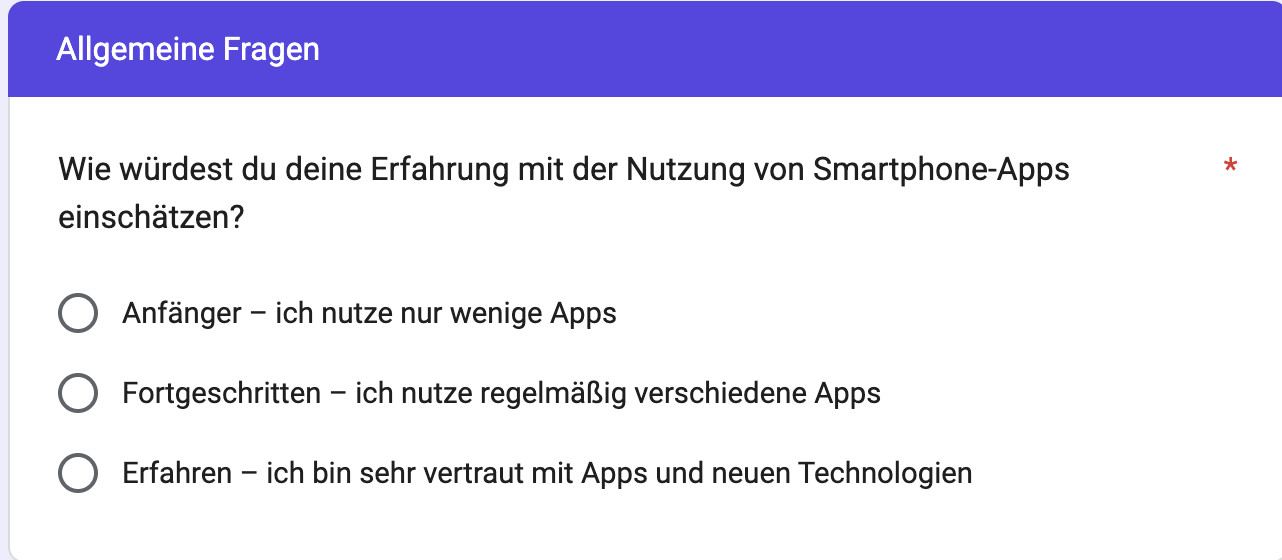
\includegraphics[width=1.0\linewidth]{figures/evaluation/allgemeine_fragen.png}
\end{figure}

\section*{Abschnitt 2: Aufgabenbezogene Fragen}

Die folgenden Fragen beziehen sich auf die vier Aufgaben der Studie.

\begin{figure}[H]
    \centering
    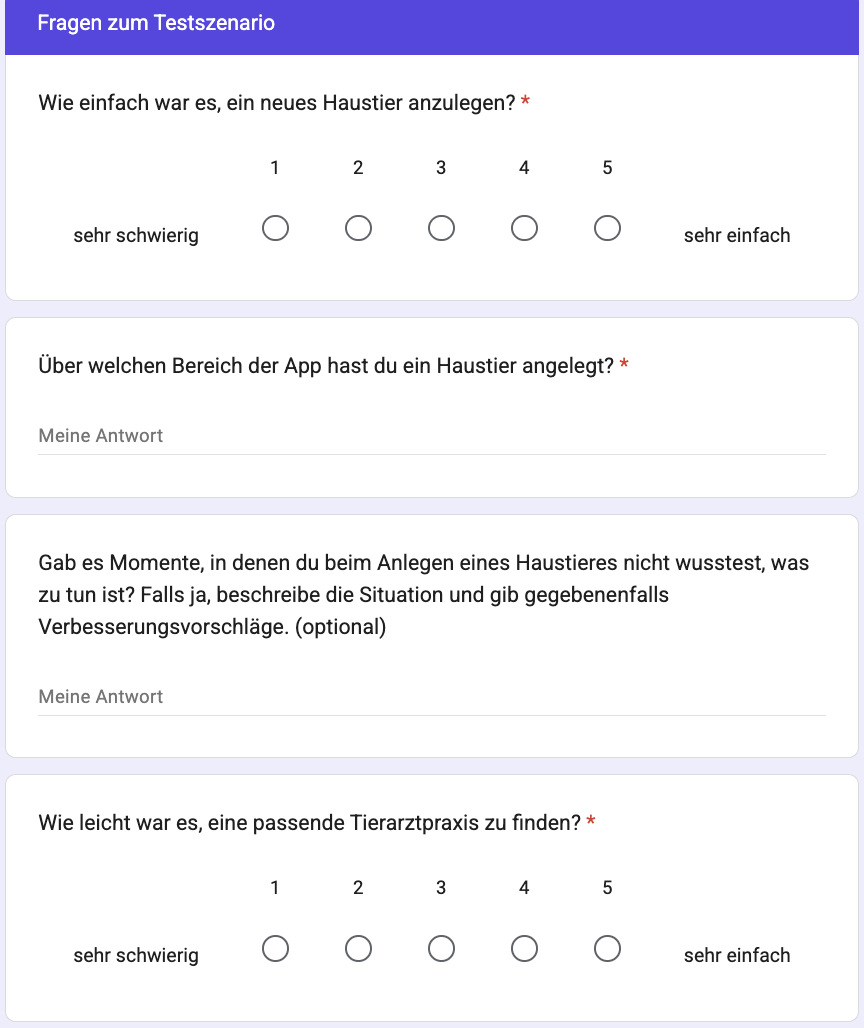
\includegraphics[width=1.0\linewidth]{figures/evaluation/Aufgaben_1.png}
\end{figure}

\begin{figure}[H]
    \centering
    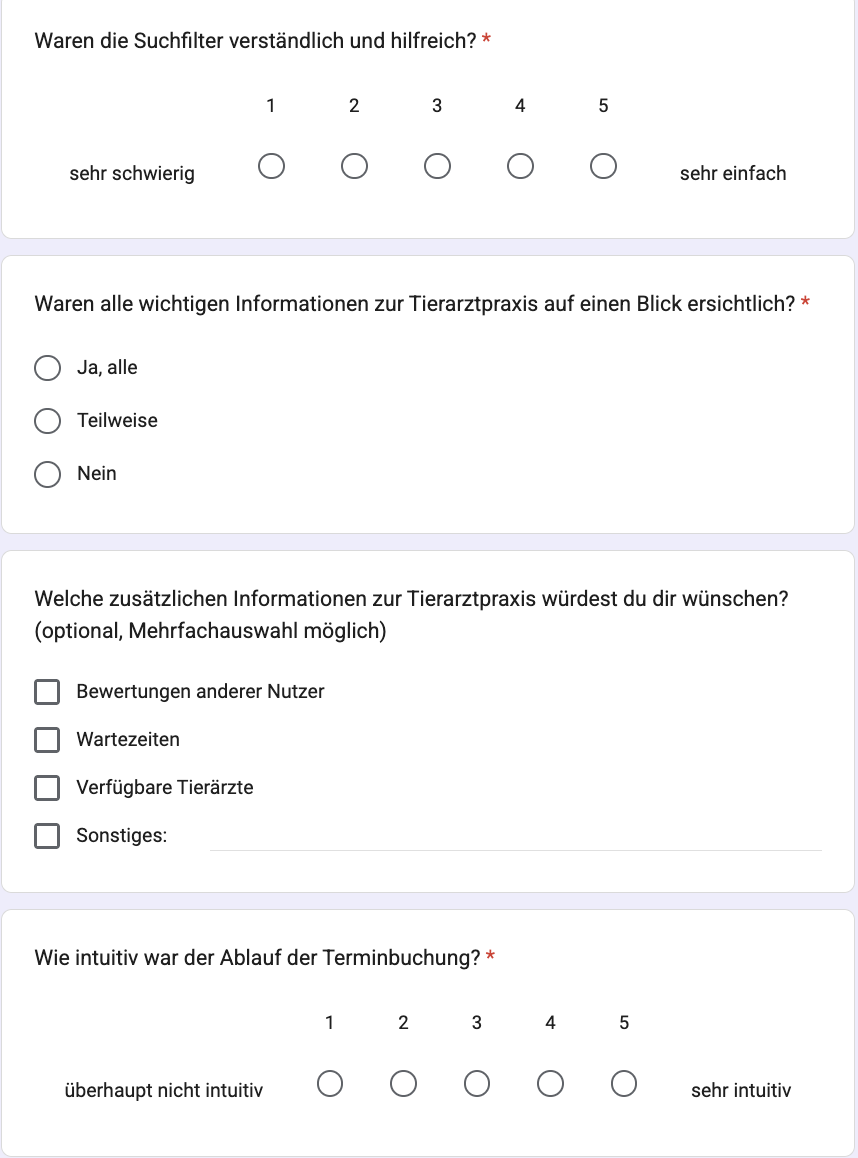
\includegraphics[width=1.0\linewidth]{figures/evaluation/Aufgaben_2.png}
\end{figure}

\begin{figure}[H]
    \centering
    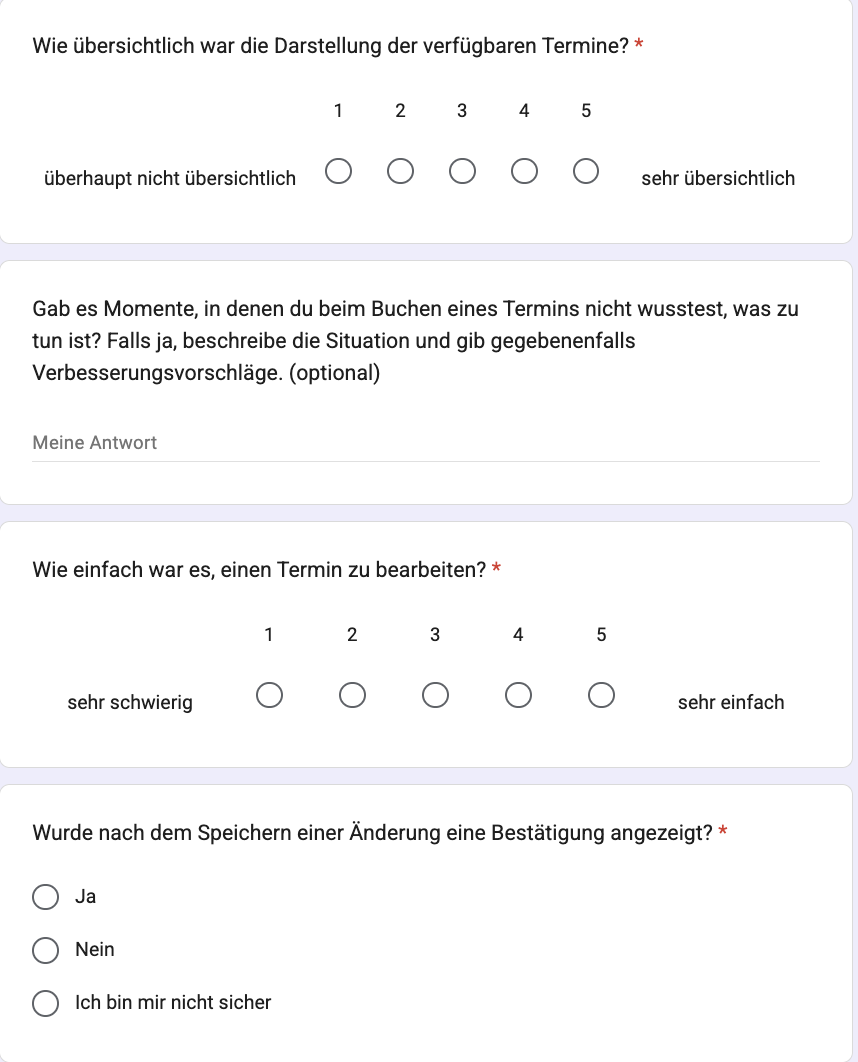
\includegraphics[width=1.0\linewidth]{figures/evaluation/Aufgaben_3.png}
\end{figure}

\begin{figure}[H]
    \centering
    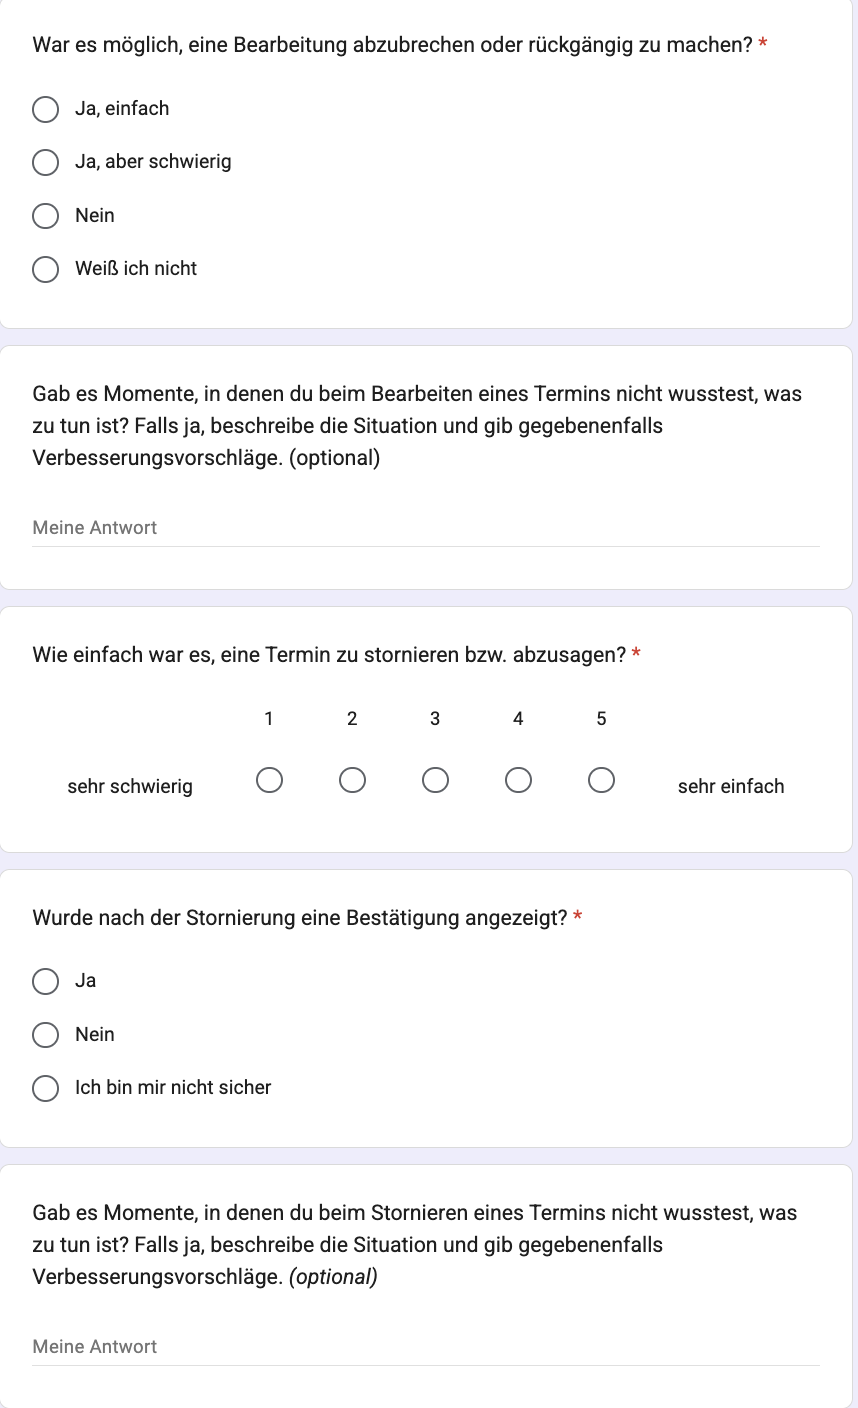
\includegraphics[width=1.0\linewidth]{figures/evaluation/Aufgaben_4.png}
\end{figure}

\section*{Abschnitt 3: System Usability Scale}

Die folgenden Fragen beziehen sich auf die Benutzerfreundlichkeit der Anwendung.

\begin{figure}[H]
    \centering
    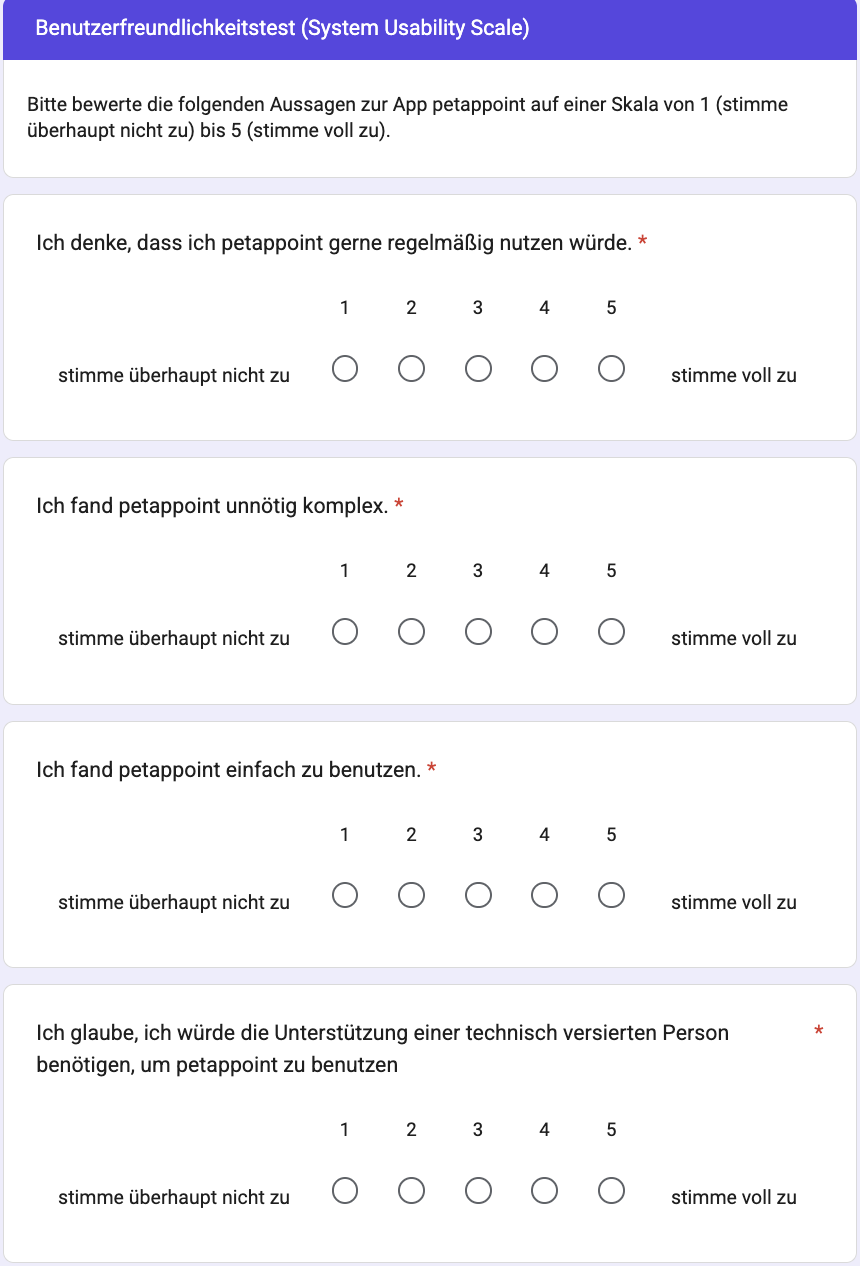
\includegraphics[width=1.0\linewidth]{figures/evaluation/Sus_1.png}
\end{figure}

\begin{figure}[H]
    \centering
    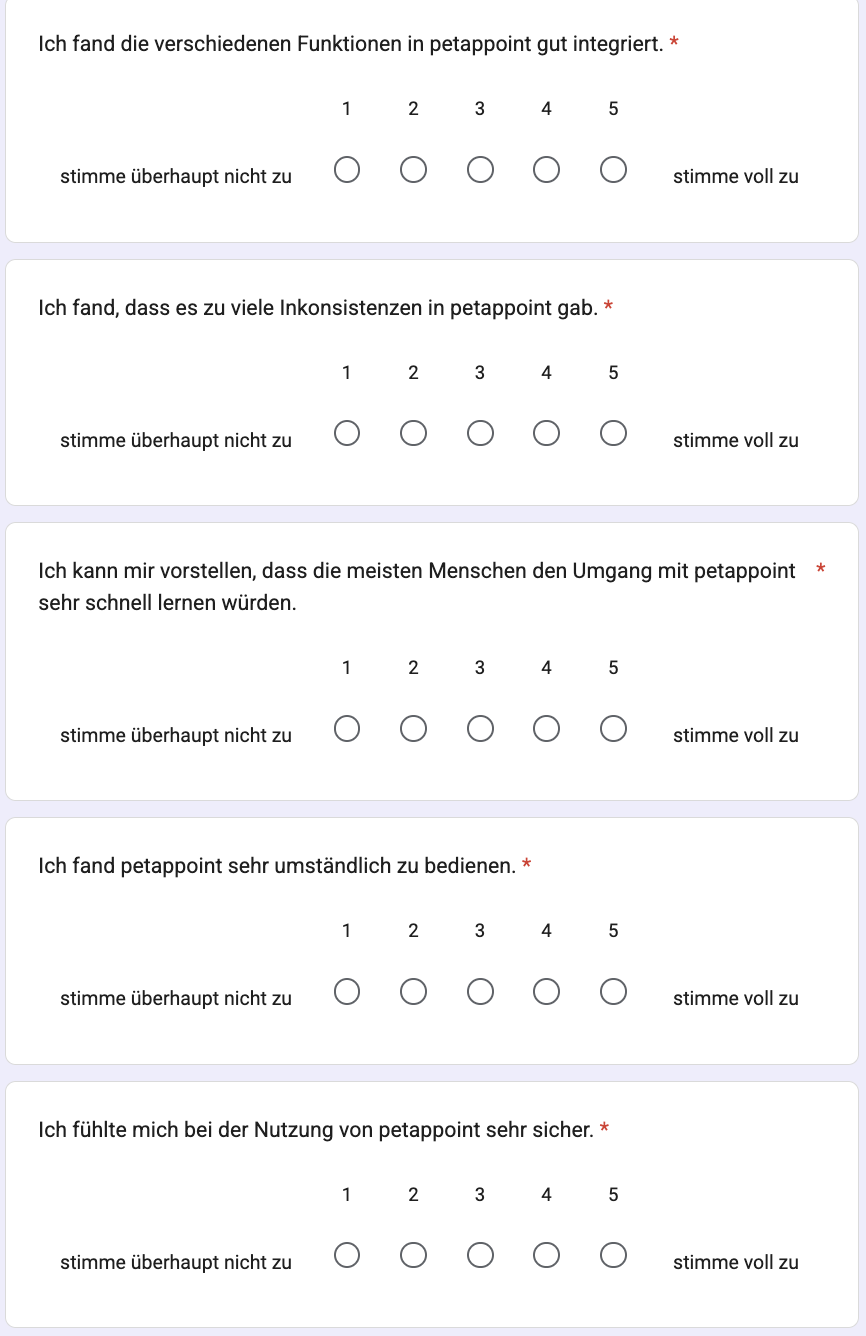
\includegraphics[width=1.0\linewidth]{figures/evaluation/Sus_2.png}
\end{figure}

\begin{figure}[H]
    \centering
    \includegraphics[width=1.0\linewidth]{figures/evaluation/Sus_3.png}
\end{figure}

\section*{Abschnitt 4: Plattformwahrnehmung}

Die folgenden Fragen beziehen sich auf die Plattformwahrnehmung der Anwendung.
\begin{figure}[H]
    \centering
    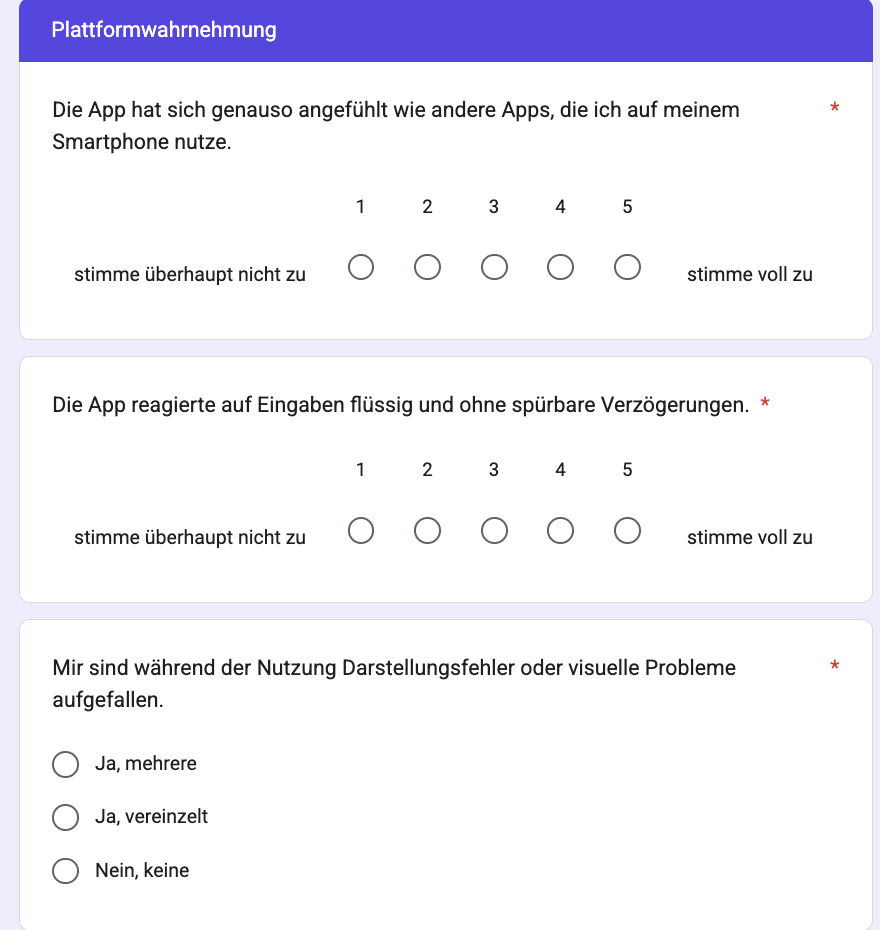
\includegraphics[width=1.0\linewidth]{figures/evaluation/Plattformwahrnehmung_1.png}
\end{figure}

\section*{Abschnitt 5: Offene Fragen}

Die folgenden offenen Fragen geben den Teilnehmenden die Möglichkeit, freies Feedback zur Anwendung zu geben.

\begin{figure}[H]
    \centering
    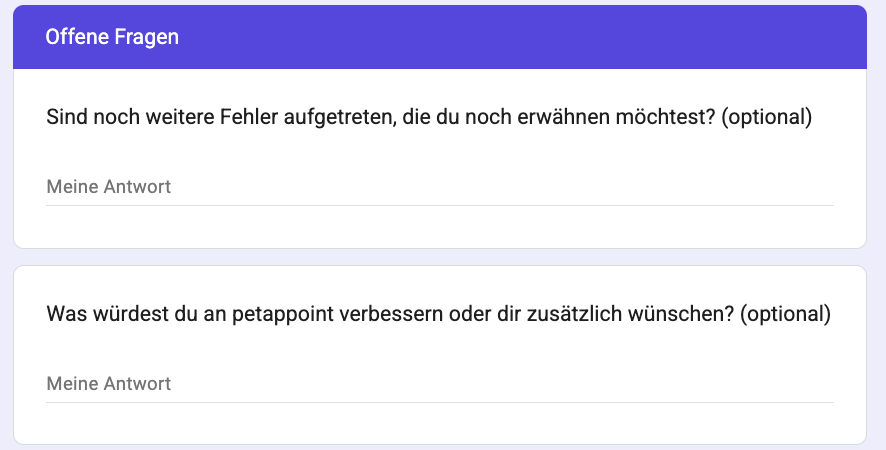
\includegraphics[width=1.0\linewidth]{figures/evaluation/offene_fragen.png}
\end{figure}


\chapter{Rohdaten der Nutzerstudie}
\label{appendix:rohdaten}
Die vollständigen Rohdaten der Nutzerstudie sind als CSV-Datei über folgenden Link abrufbar:
\begin{itemize}
  \item Fragebogenantworten (CSV): \\
\url{https://drive.google.com/file/d/1mYSi_oevs_g2PIkNzhTzI93mcST8AHD-/view?usp=sharing}
  \item Alter, Beruf und Aufgabenzeiten (Excel): \\
        \url{https://docs.google.com/spreadsheets/d/1hDo-o8bUvvBQezd9emxWkkEGwxBhKNbc/edit?usp=sharing&ouid=107616586787460661537&rtpof=true&sd=true}
  \item SUS-Scores jedes einzelnen Teilnehmer(Excel): \\
        \url{https://docs.google.com/spreadsheets/d/1hy-Kzu3R7k8lXaasbQmuu2rEZsG50OkU/edit?usp=sharing&ouid=107616586787460661537&rtpof=true&sd=true}
\end{itemize}
% \cleardoublepage

% Bibliography

\addcontentsline{toc}{chapter}{Literaturverzeichnis}
\printbibliography
\end{document}
